\appendix

\section{Additional Results}
\label{app:additional_results}

\subsection{Coinrun100k and Coinrun 2.5M Results}
Tables~\ref{tab:results_coinrun100k} and~\ref{tab:results_coinrun2500k} contain results for Coinrun datasets of different sizes (100k and 2.5M). The results in the main paper use a dataset size of 500k.
\begin{table}[h!]
\tiny
\centering
\begin{tabular}{|l|l|>{\centering\arraybackslash}p{1.1cm}|>{\centering\arraybackslash}p{1cm}|>{\centering\arraybackslash}p{1cm}|>{\centering\arraybackslash}p{1cm}|>{\centering\arraybackslash}p{1cm}|>{\centering\arraybackslash}p{1cm}|}
\hline
\rowcolor[HTML]{2A5B93} &
\textbf{\textcolor{white}{Method}} &
 \textbf{\textcolor{white}{Action Err. Ratio $\downarrow$}} &
  \textbf{\textcolor{white}{FVD $\downarrow$}} &
  \textbf{\textcolor{white}{FID $\downarrow$}} &
  \textbf{\textcolor{white}{SSIM $\uparrow$}} &
  \textbf{\textcolor{white}{LPIPS $\downarrow$}} &
  \textbf{\textcolor{white}{PSNR $\uparrow$}} 
  \\ \hline
\multirow{3}{*}{\rotatebox{90}{\textbf{Med.}}} &
  AVID (Ours) (22M) &
 \textbf{1.355} &
  \textbf{57.4} &
 10.77 &
  \textbf{0.592} &
 0.270 &
  \textbf{19.9}
 \\ 
  &   Action-Conditioned Diffusion (22M) &
    1.501 &
    65.6 &
    11.82 &
    0.487 & 
    0.365 & 
    17.2
 \\  
 &
  ControlNet-Small (22M) \shadecell &
 1.559 \shadecell &
 62.6 \shadecell &
  \textbf{10.39} \shadecell &
  \textbf{0.603} \shadecell & 
  \textbf{0.263} \shadecell &
  \textbf{20.3}  \shadecell
 \\ \hline
\multirow{3}{*}{\rotatebox{90}{\textbf{Large}}} &
  AVID (Ours) (71M) &
 \textbf{1.222} &
 \textbf{56.0} &
10.47 &
0.624 &
0.253 &
20.6
\\ 
  &  Action-Conditioned Diffusion (71M) &
  \textbf{1.224} &
 60.0 &
 11.16 &
 0.558 &
 0.312 &
 18.5
  \\ 
 &
  ControlNet (71M) \shadecell &
  1.491 \shadecell & 
57.6 \shadecell &
 \textbf{9.92} \shadecell &
 \textbf{0.697} \shadecell &
 \textbf{0.197} \shadecell & 
 \textbf{22.9}  \shadecell
 \\ \hline
\multirow{2}{*}{\rotatebox{90}{\textbf{Full}}} &
  Pretrained Base Model (97M) &
 3.855 &
 204.0 &
 13.03 &
 0.451 &
0.352 & 
17.3 
\\ 
 &
  Action-Conditioned Finetuning (97M) \shadecell &
     \textbf{1.311} \shadecell &
     \textbf{34.7} \shadecell &
     \textbf{8.38} \shadecell & 
     \textbf{0.716} \shadecell & 
     \textbf{0.167} \shadecell &
     \textbf{23.9}  \shadecell
 \\ \hline
\end{tabular}
\caption{Quantitative results for Coinrun 100k dataset. Shaded rows indicate that the method requires access to the model parameters.}
\label{tab:results_coinrun100k}
\end{table}

\begin{table}[h!]
\tiny
\centering
\begin{tabular}{|l|l|>{\centering\arraybackslash}p{1.1cm}|>{\centering\arraybackslash}p{1cm}|>{\centering\arraybackslash}p{1cm}|>{\centering\arraybackslash}p{1cm}|>{\centering\arraybackslash}p{1cm}|>{\centering\arraybackslash}p{1cm}|}
\hline
\rowcolor[HTML]{2A5B93} &
\textbf{\textcolor{white}{Method}} &
 \textbf{\textcolor{white}{Action Err. Ratio $\downarrow$}} &
  \textbf{\textcolor{white}{FVD $\downarrow$}} &
  \textbf{\textcolor{white}{FID $\downarrow$}} &
  \textbf{\textcolor{white}{SSIM $\uparrow$}} &
  \textbf{\textcolor{white}{LPIPS $\downarrow$}} &
  \textbf{\textcolor{white}{PSNR $\uparrow$}} 
  \\ \hline
\multirow{3}{*}{\rotatebox{90}{\textbf{Med.}}} &
  AVID (Ours) (22M) &
\textbf{1.277} &
24.7 &
8.01 &
\textbf{0.679} &
\textbf{0.177} &
\textbf{23.0}
 \\ 
  &   Action-Conditioned Diffusion (22M) &
1.574 &
34.8 &
8.88 &
0.580 &
0.254 &
19.4
 \\  
 &
  ControlNet-Small (22M) \shadecell &
1.467 \shadecell &
\textbf{23.8} \shadecell &
\textbf{7.80} \shadecell &
 0.653 \shadecell &
 0.194 \shadecell &
 22.1 \shadecell
 \\ \hline
\multirow{3}{*}{\rotatebox{90}{\textbf{Large}}} &
  AVID (Ours) (71M) &
\textbf{1.158} &
\textbf{14.5} &
\textbf{6.44} &
0.740 &
0.131 &
25.1 
\\ 
  &  Action-Conditioned Diffusion (71M) &
1.203 &
17.7 &
6.63 &
0.704 &
0.158 &
23.4
  \\ 
 &
  ControlNet (71M) \shadecell &
1.393 &
14.8 &
6.68 &
\textbf{0.760} &
\textbf{0.120} &
\textbf{25.7}
 \\ \hline
\multirow{2}{*}{\rotatebox{90}{\textbf{Full}}} &
Pretrained Base Model (97M) &
 3.855 &
 204.0 &
 13.03 &
 0.451 &
0.352 & 
17.3 
\\ 
 &
  Action-Conditioned Finetuning (97M) \shadecell &
  \shadecell  \textbf{1.216} &
   \shadecell \textbf{12.0} &
   \shadecell \textbf{ 6.28} &
   \shadecell \textbf{0.782} & 
  \shadecell  \textbf{0.107} &
  \shadecell  \textbf{26.6} 
 \\ \hline
\end{tabular}
\caption{Quantitative results for Coinrun 2.5M dataset. Shaded rows indicate that the method requires access to the model parameters.}
\label{tab:results_coinrun2500k}
\end{table}

\FloatBarrier

\subsection{Full Results for AVID Ablations}
\label{sec:avid_abl_full}
Table~\ref{tab:avid_abl_full} contains ablation results for AVID across the full range of model sizes.

\begin{table}[h!]
\tiny
\centering
\begin{tabular}{|l|l|>{\centering\arraybackslash}p{1.1cm}|>{\centering\arraybackslash}p{1cm}|>{\centering\arraybackslash}p{1cm}|>{\centering\arraybackslash}p{1cm}|>{\centering\arraybackslash}p{1cm}|>{\centering\arraybackslash}p{1cm}|}
\hline
\rowcolor[HTML]{2A5B93} &
\textbf{\textcolor{white}{Method}} &
 \textbf{\textcolor{white}{Action Err. Ratio $\downarrow$}} &
  \textbf{\textcolor{white}{FVD $\downarrow$}} &
  \textbf{\textcolor{white}{FID $\downarrow$}} &
  \textbf{\textcolor{white}{SSIM $\uparrow$}} &
  \textbf{\textcolor{white}{LPIPS $\downarrow$}} &
  \textbf{\textcolor{white}{PSNR $\uparrow$}} 
  \\ \hline
  \multirow{3}{*}{\rotatebox{90}{\makecell{\textbf{Coinrun} \\\textbf{500k}\\\textbf{Med.}}}}
 &
  AVID (Ours) (22M) &
 \textbf{1.257} &
 \textbf{28.5} &
 \textbf{8.07} &
 \textbf{0.666} & 
 0.192 &
22.4 \\
  & No Mask (22M) &
  \textbf{1.241} & 
  \textbf{28.6} &
 \textbf{8.06} &
  \textbf{0.675} &
  \textbf{0.186} 
&
 \textbf{22.7}
  \\ 
  & No Conditioning (22M) &
1.276 &
33.7 &
8.50 &
0.655 & 
0.208 &
21.5\\ \hline
  \multirow{3}{*}{\rotatebox{90}{\makecell{\textbf{Coinrun}\\\textbf{500k}\\\textbf{Large}}}}
 &
  AVID (Ours) (71M)  &
  \textbf{1.154} &
23.1 &
7.33 & 
\textbf{0.713} &
\textbf{0.161} &
\textbf{23.8} \\ 
  & No Mask (71M) &
  \textbf{1.136} &
  \textbf{22.2} & 
  \textbf{7.15} & 
  \textbf{0.721} &
  \textbf{0.158} &
  \textbf{24.0}
  \\ 
  & No Conditioning (71M) &
   \textbf{1.141} &
  27.8 &
  8.02 &
  0.682 & 
  0.189 &
  22.3
 \\ \hline
  \multirow{3}{*}{\rotatebox{90}{\makecell{\textbf{RT1}\\\textbf{Small}}}}
 &
  AVID (Ours) (11M) &
  \textbf{2.572} &
  \textbf{54.0} &
  \textbf{4.344} &
  \textbf{0.811} &
  \textbf{0.166} & 
  \textbf{24.5} \\ 
  &
  No Mask (11M) &
  2.752 &
  63.7 &
  4.566 &
  \textbf{0.809} &
  \textbf{0.168} &
  23.8
  \\
  & No Conditioning (11M) &
 2.938 &
 60.5 &
 4.620 &
  \textbf{0.806} & 
0.172 &
  \textbf{24.5} \\ \hline
\multirow{3}{*}{\rotatebox{90}{\makecell{\textbf{RT1}\\\textbf{Med.}}}}
 &
  AVID (Ours) (34M) &
  \textbf{1.907}  &
  \textbf{38.7} &
  \textbf{3.645} &
  \textbf{0.831} &
  \textbf{0.150} &
  \textbf{25.0} \\ 
  &
  No Mask (34M) &
  2.155  &
  49.7 &
  3.940 &
  \textbf{0.825} &
  0.156 &
  24.5 \\ 
  & No Conditioning (34M) &
  2.349 &
  48.6 &
  4.018 &
  \textbf{0.819} &
  0.160 &
  \textbf{25.1}
 \\ \hline
 \multirow{3}{*}{\rotatebox{90}{\makecell{\textbf{RT1}\\\textbf{Large}}}}
 &
  AVID (Ours) (145M) &
  \textbf{1.609} &
  39.3 &
  \textbf{3.436} &
  \textbf{0.842} &
  \textbf{0.142} &
  \textbf{25.3} \\ 
 &
  No Mask (145M) &
  1.769 &
  44.1 &
  3.533 &
  \textbf{0.836} &
  0.146 &
  \textbf{25.3} \\ 
  & No Conditioning (145M) &
  1.775 &
  \textbf{36.2} &
  3.550 & 
  \textbf{0.827} &
  0.149 &
  25.0 
 \\ \hline
\end{tabular}
\caption{Full results for AVID ablations.}
\label{tab:avid_abl_full}
\end{table}

\subsection{RT1 Results with Larger Compute Limit}
The results in the main paper train models for RT1 using a compute limit of 7 days of 4$\times$ A100 GPUs.
To provide reference values for performance we also evaluated IRASim~\citep{zhu2024irasim} using our evaluation setup. IRASim is a 679M parameter model trained using 100 GPU-days on A800 GPUs.
%
We also include results for action-conditioned finetuning of DynamiCrafter using a similar amount of compute (104 GPU-days on A100 GPUs).
%
The results for these two models are in Table~\ref{tab:high_compute}.
%
By finetuning DynamiCrafter, we obtain slightly stronger performance than IRASim.

\begin{table}[h!]
\tiny
\centering
\begin{tabular}{|l|>{\centering\arraybackslash}p{1.1cm}|>{\centering\arraybackslash}p{1cm}|>{\centering\arraybackslash}p{1cm}|>{\centering\arraybackslash}p{1cm}|>{\centering\arraybackslash}p{1cm}|>{\centering\arraybackslash}p{1cm}|}
\hline
\rowcolor[HTML]{2A5B93} 
\textbf{\textcolor{white}{Method}} &
 \textbf{\textcolor{white}{Action Err. Ratio $\downarrow$}} &
  \textbf{\textcolor{white}{FVD $\downarrow$}} &
  \textbf{\textcolor{white}{FID $\downarrow$}} &
  \textbf{\textcolor{white}{SSIM $\uparrow$}} &
  \textbf{\textcolor{white}{LPIPS $\downarrow$}} &
  \textbf{\textcolor{white}{PSNR $\uparrow$}} 
  \\ \hline
  IRASim  &
   - &
   21.0 &
   2.759 &
   0.879 &
   0.1296 &
   28.2 \\ 
  Action-Conditioned Finetuning (1.4B)  &
   1.151 &
   19.5 &
   2.655 &
    0.871 &
    0.1160
    & 27.1\\  \hline
\end{tabular}
\caption{Quantitative results for RT1 dataset with greater computational budget. }
\label{tab:high_compute}
\end{table}

\FloatBarrier

\subsection{Examples of AVID Masking}
\label{app:masking}
Figures~\ref{fig:procgen_mask} and~\ref{fig:rt1_mask} illustrate examples of the mask generated by AVID which is used to mix the pretrained model and adapter outputs.

\begin{figure}[htbp]
    %
    \begin{minipage}{0.05\textwidth} % Column for rotated method name
        \centering
        \raisebox{0.3\textwidth}{\rotatebox{90}{\textbf{\tiny AVID 71M}}} % Rotating and vertically centering method name
    \end{minipage}%
    \hfill
    \begin{minipage}{0.13\textwidth}
        \centering
        
\includegraphics[width=\textwidth]{images/coinrun/avid_71M/3-424_frames/frame_2.png}
    \end{minipage}%
    \hfill
    \begin{minipage}{0.13\textwidth}
        \centering
        
\includegraphics[width=\textwidth]{images/coinrun/avid_71M/3-424_frames/frame_3.png}
    \end{minipage}%
    \hfill
    \begin{minipage}{0.13\textwidth}
        \centering
        
\includegraphics[width=\textwidth]{images/coinrun/avid_71M/3-424_frames/frame_4.png}
    \end{minipage}%
    \hfill
    \begin{minipage}{0.13\textwidth}
        \centering
        
\includegraphics[width=\textwidth]{images/coinrun/avid_71M/3-424_frames/frame_5.png}
    \end{minipage}%
    \hfill
    \begin{minipage}{0.13\textwidth}
        \centering
        
\includegraphics[width=\textwidth]{images/coinrun/avid_71M/3-424_frames/frame_7.png}
    \end{minipage}%
    \hfill
    \begin{minipage}{0.13\textwidth}
        \centering
        
\includegraphics[width=\textwidth]{images/coinrun/avid_71M/3-424_frames/frame_8.png}
    \end{minipage}%
    \hfill
    \begin{minipage}{0.13\textwidth}
        \centering
        
\includegraphics[width=\textwidth]{images/coinrun/avid_71M/3-424_frames/frame_9.png}
    \end{minipage}%
    \vspace{0.01cm}
    %
    \begin{minipage}{0.05\textwidth} % Column for rotated method name
        \centering
        \raisebox{0.1\textwidth}{\rotatebox{90}{\textbf{\tiny \shortstack{Mask}}}}
    \end{minipage}%
    \hfill
    \begin{minipage}{0.13\textwidth}
        \centering
        
\includegraphics[width=\textwidth]{images/masking/coinrun_avid_71M/3-424_frames/frame_1.png}
    \end{minipage}%
    \hfill
    \begin{minipage}{0.13\textwidth}
        \centering
        
\includegraphics[width=\textwidth]{images/masking/coinrun_avid_71M/3-424_frames/frame_2.png}
    \end{minipage}%
    \hfill
    \begin{minipage}{0.13\textwidth}
        \centering
        
\includegraphics[width=\textwidth]{images/masking/coinrun_avid_71M/3-424_frames/frame_3.png}
    \end{minipage}%
    \hfill
    \begin{minipage}{0.13\textwidth}
        \centering
        
\includegraphics[width=\textwidth]{images/masking/coinrun_avid_71M/3-424_frames/frame_4.png}
    \end{minipage}%
    \hfill
    \begin{minipage}{0.13\textwidth}
        \centering
        
\includegraphics[width=\textwidth]{images/masking/coinrun_avid_71M/3-424_frames/frame_6.png}
    \end{minipage}%
    \hfill
    \begin{minipage}{0.13\textwidth}
        \centering
        
\includegraphics[width=\textwidth]{images/masking/coinrun_avid_71M/3-424_frames/frame_7.png}
    \end{minipage}%
    \hfill
    \begin{minipage}{0.13\textwidth}
        \centering
        
\includegraphics[width=\textwidth]{images/masking/coinrun_avid_71M/3-424_frames/frame_8.png}
    \end{minipage}%
    %
    %
    \vspace{0.2cm}
    %
    %
    %
    \begin{minipage}{0.05\textwidth} % Column for rotated method name
        \centering
        \raisebox{0.3\textwidth}{\rotatebox{90}{\textbf{\tiny AVID 71M}}} % Rotating and vertically centering method name
    \end{minipage}%
    \hfill
    \begin{minipage}{0.13\textwidth}
        \centering
        
\includegraphics[width=\textwidth]{images/coinrun/avid_71M/2-837_frames/frame_2.png}
    \end{minipage}%
    \hfill
    \begin{minipage}{0.13\textwidth}
        \centering
        
\includegraphics[width=\textwidth]{images/coinrun/avid_71M/2-837_frames/frame_3.png}
    \end{minipage}%
    \hfill
    \begin{minipage}{0.13\textwidth}
        \centering
        
\includegraphics[width=\textwidth]{images/coinrun/avid_71M/2-837_frames/frame_4.png}
    \end{minipage}%
    \hfill
    \begin{minipage}{0.13\textwidth}
        \centering
        
\includegraphics[width=\textwidth]{images/coinrun/avid_71M/2-837_frames/frame_5.png}
    \end{minipage}%
    \hfill
    \begin{minipage}{0.13\textwidth}
        \centering
        
\includegraphics[width=\textwidth]{images/coinrun/avid_71M/2-837_frames/frame_7.png}
    \end{minipage}%
    \hfill
    \begin{minipage}{0.13\textwidth}
        \centering
        
\includegraphics[width=\textwidth]{images/coinrun/avid_71M/2-837_frames/frame_8.png}
    \end{minipage}%
    \hfill
    \begin{minipage}{0.13\textwidth}
        \centering
        
\includegraphics[width=\textwidth]{images/coinrun/avid_71M/2-837_frames/frame_9.png}
    \end{minipage}%
    \vspace{0.01cm}
    %
    \begin{minipage}{0.05\textwidth} % Column for rotated method name
        \centering
        \raisebox{0.1\textwidth}{\rotatebox{90}{\textbf{\tiny \shortstack{Mask}}}}
    \end{minipage}%
    \hfill
    \begin{minipage}{0.13\textwidth}
        \centering
        
\includegraphics[width=\textwidth]{images/masking/coinrun_avid_71M/2-837_frames/frame_1.png}
    \end{minipage}%
    \hfill
    \begin{minipage}{0.13\textwidth}
        \centering
        
\includegraphics[width=\textwidth]{images/masking/coinrun_avid_71M/2-837_frames/frame_2.png}
    \end{minipage}%
    \hfill
    \begin{minipage}{0.13\textwidth}
        \centering
        
\includegraphics[width=\textwidth]{images/masking/coinrun_avid_71M/2-837_frames/frame_3.png}
    \end{minipage}%
    \hfill
    \begin{minipage}{0.13\textwidth}
        \centering
        
\includegraphics[width=\textwidth]{images/masking/coinrun_avid_71M/2-837_frames/frame_4.png}
    \end{minipage}%
    \hfill
    \begin{minipage}{0.13\textwidth}
        \centering
        
\includegraphics[width=\textwidth]{images/masking/coinrun_avid_71M/2-837_frames/frame_6.png}
    \end{minipage}%
    \hfill
    \begin{minipage}{0.13\textwidth}
        \centering
        
\includegraphics[width=\textwidth]{images/masking/coinrun_avid_71M/2-837_frames/frame_7.png}
    \end{minipage}%
    \hfill
    \begin{minipage}{0.13\textwidth}
        \centering
        
\includegraphics[width=\textwidth]{images/masking/coinrun_avid_71M/2-837_frames/frame_8.png}
    \end{minipage}%
    \caption{Examples of the mask, $m$, produced by AVID averaged throughout the diffusion process for Coinrun500k. White indicates the mask is set to 1, and black indicates the mask is set to 0. \label{fig:procgen_mask}}
\end{figure}


\begin{figure}[htbp]
    \centering
    % Row 1
    \begin{minipage}{0.04\textwidth} % Column for rotated method name
        \centering
        \raisebox{0.3\textwidth}{\rotatebox{90}{\textbf{\tiny AVID 145M}}} % Rotating and vertically centering method name
    \end{minipage}%
    \hfill
    \begin{minipage}{0.155\textwidth}
        \centering
        
\includegraphics[width=\textwidth]{images/rt1/avid_145M/3-28-samples_frames/frame_0.png}
    \end{minipage}%
    \hfill
    \begin{minipage}{0.155\textwidth}
        \centering
        
\includegraphics[width=\textwidth]{images/rt1/avid_145M/3-28-samples_frames/frame_3.png}
    \end{minipage}%
    \hfill
    \begin{minipage}{0.155\textwidth}
        \centering
        
\includegraphics[width=\textwidth]{images/rt1/avid_145M/3-28-samples_frames/frame_6.png}
    \end{minipage}%
    \hfill
    \begin{minipage}{0.155\textwidth}
        \centering
        
\includegraphics[width=\textwidth]{images/rt1/avid_145M/3-28-samples_frames/frame_9.png}
    \end{minipage}%
    \hfill
    \begin{minipage}{0.155\textwidth}
        \centering
        
\includegraphics[width=\textwidth]{images/rt1/avid_145M/3-28-samples_frames/frame_12.png}
    \end{minipage}%
    \hfill
    \begin{minipage}{0.155\textwidth}
        \centering
        
\includegraphics[width=\textwidth]{images/rt1/avid_145M/3-28-samples_frames/frame_15.png}
    \end{minipage}%
    \vspace{0.03cm} % Space between rows
   \begin{minipage}{0.04\textwidth} % Column for rotated method name
        \centering
        \raisebox{0.2\textwidth}{\rotatebox{90}{\textbf{\tiny Latent Mask}}} % Rotating and vertically centering method name
    \end{minipage}%
    \hfill
    \begin{minipage}{0.155\textwidth}
        \centering
        
\includegraphics[width=\textwidth]{images/masking/rt1_avid_145M/3-28-mask_frames/frame_0.png}
    \end{minipage}%
    \hfill
    \begin{minipage}{0.155\textwidth}
        \centering
        
\includegraphics[width=\textwidth]{images/masking/rt1_avid_145M/3-28-mask_frames/frame_3.png}
    \end{minipage}%
    \hfill
    \begin{minipage}{0.155\textwidth}
        \centering
        
\includegraphics[width=\textwidth]{images/masking/rt1_avid_145M/3-28-mask_frames/frame_6.png}
    \end{minipage}%
    \hfill
    \begin{minipage}{0.155\textwidth}
        \centering
        
\includegraphics[width=\textwidth]{images/masking/rt1_avid_145M/3-28-mask_frames/frame_9.png}
    \end{minipage}%
    \hfill
    \begin{minipage}{0.155\textwidth}
        \centering
        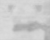
\includegraphics[width=\textwidth]{images/masking/rt1_avid_145M/3-28-mask_frames/frame_12.png}
    \end{minipage}%
    \hfill
    \begin{minipage}{0.155\textwidth}
        \centering
        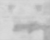
\includegraphics[width=\textwidth]{images/masking/rt1_avid_145M/3-28-mask_frames/frame_15.png}
    \end{minipage}%
    %
    %
    \vspace{0.2cm} % Space between rows
    %
    %
    \begin{minipage}{0.04\textwidth} % Column for rotated method name
        \centering
        \raisebox{0.3\textwidth}{\rotatebox{90}{\textbf{\tiny AVID 145M}}} % Rotating and vertically centering method name
    \end{minipage}%
    \hfill
    \begin{minipage}{0.155\textwidth}
        \centering
        
\includegraphics[width=\textwidth]{images/rt1/avid_145M/3-70-samples_frames/frame_0.png}
    \end{minipage}%
    \hfill
    \begin{minipage}{0.155\textwidth}
        \centering
        
\includegraphics[width=\textwidth]{images/rt1/avid_145M/3-70-samples_frames/frame_3.png}
    \end{minipage}%
    \hfill
    \begin{minipage}{0.155\textwidth}
        \centering
        
\includegraphics[width=\textwidth]{images/rt1/avid_145M/3-70-samples_frames/frame_6.png}
    \end{minipage}%
    \hfill
    \begin{minipage}{0.155\textwidth}
        \centering
        
\includegraphics[width=\textwidth]{images/rt1/avid_145M/3-70-samples_frames/frame_9.png}
    \end{minipage}%
    \hfill
    \begin{minipage}{0.155\textwidth}
        \centering
        
\includegraphics[width=\textwidth]{images/rt1/avid_145M/3-70-samples_frames/frame_12.png}
    \end{minipage}%
    \hfill
    \begin{minipage}{0.155\textwidth}
        \centering
        
\includegraphics[width=\textwidth]{images/rt1/avid_145M/3-70-samples_frames/frame_15.png}
    \end{minipage}%
    \vspace{0.03cm} % Space between rows
   \begin{minipage}{0.04\textwidth} % Column for rotated method name
        \centering
        \raisebox{0.2\textwidth}{\rotatebox{90}{\textbf{\tiny Latent Mask}}} % Rotating and vertically centering method name
    \end{minipage}%
    \hfill
    \begin{minipage}{0.155\textwidth}
        \centering
        
\includegraphics[width=\textwidth]{images/masking/rt1_avid_145M/3-70-mask_frames/frame_0.png}
    \end{minipage}%
    \hfill
    \begin{minipage}{0.155\textwidth}
        \centering
        
\includegraphics[width=\textwidth]{images/masking/rt1_avid_145M/3-70-mask_frames/frame_3.png}
    \end{minipage}%
    \hfill
    \begin{minipage}{0.155\textwidth}
        \centering
        
\includegraphics[width=\textwidth]{images/masking/rt1_avid_145M/3-70-mask_frames/frame_6.png}
    \end{minipage}%
    \hfill
    \begin{minipage}{0.155\textwidth}
        \centering
        
\includegraphics[width=\textwidth]{images/masking/rt1_avid_145M/3-70-mask_frames/frame_9.png}
    \end{minipage}%
    \hfill
    \begin{minipage}{0.155\textwidth}
        \centering
        
\includegraphics[width=\textwidth]{images/masking/rt1_avid_145M/3-70-mask_frames/frame_12.png}
    \end{minipage}%
    \hfill
    \begin{minipage}{0.155\textwidth}
        \centering
        
\includegraphics[width=\textwidth]{images/masking/rt1_avid_145M/3-70-mask_frames/frame_15.png}
    \end{minipage}%
    \caption{Examples of the mask, $m$, produced by AVID averaged throughout the diffusion process for RT1. Note that the mask is in the latent space, where the images have been downsampled by a factor of 8. White indicates the mask is set to 1, and black indicates the mask is set to 0. \label{fig:rt1_mask}}
\end{figure}

\subsection{Extended Qualitative Examples}
\label{app:qualitative}

\begin{figure}[htbp]
    \centering
    % Row 1
    \begin{minipage}{0.04\textwidth} % Column for rotated method name
        \centering
        \raisebox{0.3\textwidth}{\rotatebox{90}{\textbf{\tiny Ground Truth}}} % Rotating and vertically centering method name
    \end{minipage}%
    \hfill
    \begin{minipage}{0.155\textwidth}
        \centering
        
\includegraphics[width=\textwidth]{images/rt1/real_videos/3-70-real_frames/frame_0.png}
    \end{minipage}%
    \hfill
    \begin{minipage}{0.155\textwidth}
        \centering
        
\includegraphics[width=\textwidth]{images/rt1/real_videos/3-70-real_frames/frame_3.png}
    \end{minipage}%
    \hfill
    \begin{minipage}{0.155\textwidth}
        \centering
        
\includegraphics[width=\textwidth]{images/rt1/real_videos/3-70-real_frames/frame_6.png}
    \end{minipage}%
    \hfill
    \begin{minipage}{0.155\textwidth}
        \centering
        
\includegraphics[width=\textwidth]{images/rt1/real_videos/3-70-real_frames/frame_9.png}
    \end{minipage}%
    \hfill
    \begin{minipage}{0.155\textwidth}
        \centering
        
\includegraphics[width=\textwidth]{images/rt1/real_videos/3-70-real_frames/frame_12.png}
    \end{minipage}%
    \hfill
    \begin{minipage}{0.155\textwidth}
        \centering
        
\includegraphics[width=\textwidth]{images/rt1/real_videos/3-70-real_frames/frame_15.png}
    \end{minipage}%
    \vspace{0.03cm} % Space between rows
   \begin{minipage}{0.04\textwidth} % Column for rotated method name
        \centering
        \raisebox{0.3\textwidth}{\rotatebox{90}{\textbf{\tiny AVID 145M}}} % Rotating and vertically centering method name
    \end{minipage}%
    \hfill
    \begin{minipage}{0.155\textwidth}
        \centering
        
\includegraphics[width=\textwidth]{images/rt1/avid_145M/3-70-samples_frames/frame_0.png}
    \end{minipage}%
    \hfill
    \begin{minipage}{0.155\textwidth}
        \centering
        
\includegraphics[width=\textwidth]{images/rt1/avid_145M/3-70-samples_frames/frame_3.png}
    \end{minipage}%
    \hfill
    \begin{minipage}{0.155\textwidth}
        \centering
        
\includegraphics[width=\textwidth]{images/rt1/avid_145M/3-70-samples_frames/frame_6.png}
    \end{minipage}%
    \hfill
    \begin{minipage}{0.155\textwidth}
        \centering
        
\includegraphics[width=\textwidth]{images/rt1/avid_145M/3-70-samples_frames/frame_9.png}
    \end{minipage}%
    \hfill
    \begin{minipage}{0.155\textwidth}
        \centering
        
\includegraphics[width=\textwidth]{images/rt1/avid_145M/3-70-samples_frames/frame_12.png}
    \end{minipage}%
    \hfill
    \begin{minipage}{0.155\textwidth}
        \centering
        
\includegraphics[width=\textwidth]{images/rt1/avid_145M/3-70-samples_frames/frame_15.png}
    \end{minipage}%
    \vspace{0.03cm} % Space between rows
    \begin{minipage}{0.04\textwidth} % Column for rotated method name
        \centering
        \raisebox{0.1\textwidth}{\rotatebox{90}{\textbf{\tiny \shortstack{Action Cond.\\Diffusion 145M }}}}
    \end{minipage}%
    \hfill
    \begin{minipage}{0.155\textwidth}
        \centering
        
\includegraphics[width=\textwidth]{images/rt1/act_cond_diffusion_145M/3-70-samples_frames/frame_0.png}
    \end{minipage}%
    \hfill
    \begin{minipage}{0.155\textwidth}
        \centering
        
\includegraphics[width=\textwidth]{images/rt1/act_cond_diffusion_145M/3-70-samples_frames/frame_3.png}
    \end{minipage}%
    \hfill
    \begin{minipage}{0.155\textwidth}
        \centering
        
\includegraphics[width=\textwidth]{images/rt1/act_cond_diffusion_145M/3-70-samples_frames/frame_6.png}
    \end{minipage}%
    \hfill
    \begin{minipage}{0.155\textwidth}
        \centering
        
\includegraphics[width=\textwidth]{images/rt1/act_cond_diffusion_145M/3-70-samples_frames/frame_9.png}
    \end{minipage}%
    \hfill
    \begin{minipage}{0.155\textwidth}
        \centering
        
\includegraphics[width=\textwidth]{images/rt1/act_cond_diffusion_145M/3-70-samples_frames/frame_12.png}
    \end{minipage}%
    \hfill
    \begin{minipage}{0.155\textwidth}
        \centering
        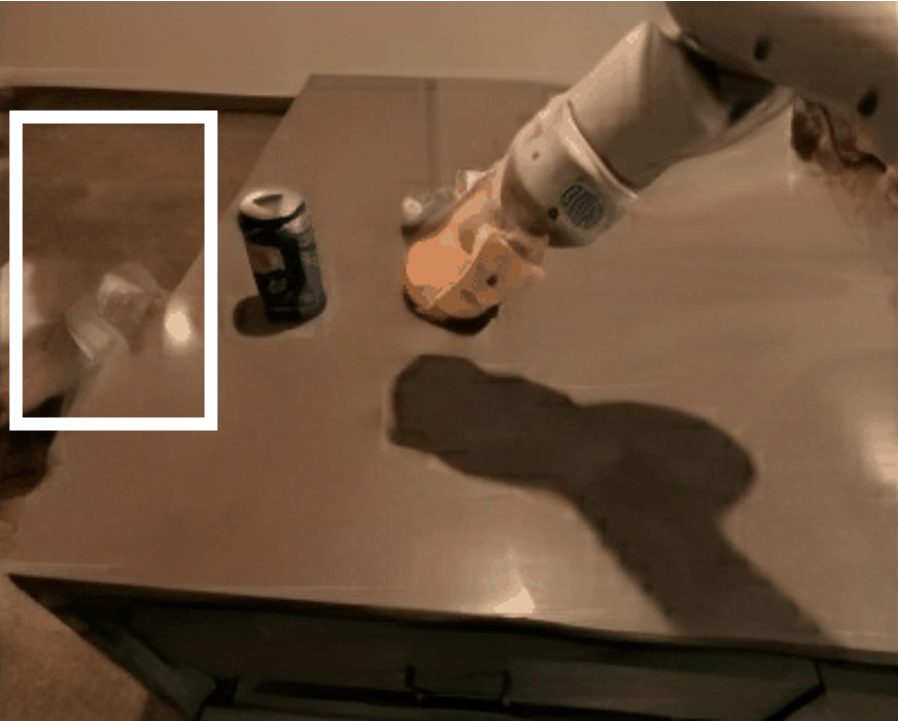
\includegraphics[width=\textwidth]{images/rt1/edited_frames/3-70_act_cond_145M_final_frame.png}
    \end{minipage}%
    \vspace{0.03cm}
    \begin{minipage}{0.04\textwidth} % Column for rotated method name
        \centering
        \raisebox{0.1\textwidth}{\rotatebox{90}{\textbf{\tiny \shortstack{DynamiCrafter }}}}
    \end{minipage}%
    \hfill
    \begin{minipage}{0.155\textwidth}
        \centering
        
\includegraphics[width=\textwidth]{images/rt1/dynamicrafter/3-70-samples_frames/frame_0.png}
    \end{minipage}%
    \hfill
    \begin{minipage}{0.155\textwidth}
        \centering
        
\includegraphics[width=\textwidth]{images/rt1/dynamicrafter/3-70-samples_frames/frame_3.png}
    \end{minipage}%
    \hfill
    \begin{minipage}{0.155\textwidth}
        \centering
        
\includegraphics[width=\textwidth]{images/rt1/dynamicrafter/3-70-samples_frames/frame_6.png}
    \end{minipage}%
    \hfill
    \begin{minipage}{0.155\textwidth}
        \centering
        
\includegraphics[width=\textwidth]{images/rt1/dynamicrafter/3-70-samples_frames/frame_9.png}
    \end{minipage}%
    \hfill
    \begin{minipage}{0.155\textwidth}
        \centering
        
\includegraphics[width=\textwidth]{images/rt1/dynamicrafter/3-70-samples_frames/frame_12.png}
    \end{minipage}%
    \hfill
    \begin{minipage}{0.155\textwidth}
        \centering
        
\includegraphics[width=\textwidth]{images/rt1/dynamicrafter/3-70-samples_frames/frame_15.png}
    \end{minipage}%
    \vspace{0.4cm}
    \begin{minipage}{0.04\textwidth} % Column for rotated method name
        \centering
        \raisebox{0.3\textwidth}{\rotatebox{90}{\textbf{\tiny Ground Truth}}} % Rotating and vertically centering method name
    \end{minipage}%
    \hfill
    \begin{minipage}{0.155\textwidth}
        \centering
        
\includegraphics[width=\textwidth]{images/rt1/real_videos/3-28-real_frames/frame_0.png}
    \end{minipage}%
    \hfill
    \begin{minipage}{0.155\textwidth}
        \centering
        
\includegraphics[width=\textwidth]{images/rt1/real_videos/3-28-real_frames/frame_3.png}
    \end{minipage}%
    \hfill
    \begin{minipage}{0.155\textwidth}
        \centering
        
\includegraphics[width=\textwidth]{images/rt1/real_videos/3-28-real_frames/frame_6.png}
    \end{minipage}%
    \hfill
    \begin{minipage}{0.155\textwidth}
        \centering
        
\includegraphics[width=\textwidth]{images/rt1/real_videos/3-28-real_frames/frame_9.png}
    \end{minipage}%
    \hfill
    \begin{minipage}{0.155\textwidth}
        \centering
        
\includegraphics[width=\textwidth]{images/rt1/real_videos/3-28-real_frames/frame_12.png}
    \end{minipage}%
    \hfill
    \begin{minipage}{0.155\textwidth}
        \centering
        
\includegraphics[width=\textwidth]{images/rt1/real_videos/3-28-real_frames/frame_15.png}
    \end{minipage}%
    \vspace{0.03cm} % Space between rows
   \begin{minipage}{0.04\textwidth} % Column for rotated method name
        \centering
        \raisebox{0.3\textwidth}{\rotatebox{90}{\textbf{\tiny AVID 145M}}} % Rotating and vertically centering method name
    \end{minipage}%
    \hfill
    \begin{minipage}{0.155\textwidth}
        \centering
        
\includegraphics[width=\textwidth]{images/rt1/avid_145M/3-28-samples_frames/frame_0.png}
    \end{minipage}%
    \hfill
    \begin{minipage}{0.155\textwidth}
        \centering
        
\includegraphics[width=\textwidth]{images/rt1/avid_145M/3-28-samples_frames/frame_3.png}
    \end{minipage}%
    \hfill
    \begin{minipage}{0.155\textwidth}
        \centering
        
\includegraphics[width=\textwidth]{images/rt1/avid_145M/3-28-samples_frames/frame_6.png}
    \end{minipage}%
    \hfill
    \begin{minipage}{0.155\textwidth}
        \centering
        
\includegraphics[width=\textwidth]{images/rt1/avid_145M/3-28-samples_frames/frame_9.png}
    \end{minipage}%
    \hfill
    \begin{minipage}{0.155\textwidth}
        \centering
        
\includegraphics[width=\textwidth]{images/rt1/avid_145M/3-28-samples_frames/frame_12.png}
    \end{minipage}%
    \hfill
    \begin{minipage}{0.155\textwidth}
        \centering
        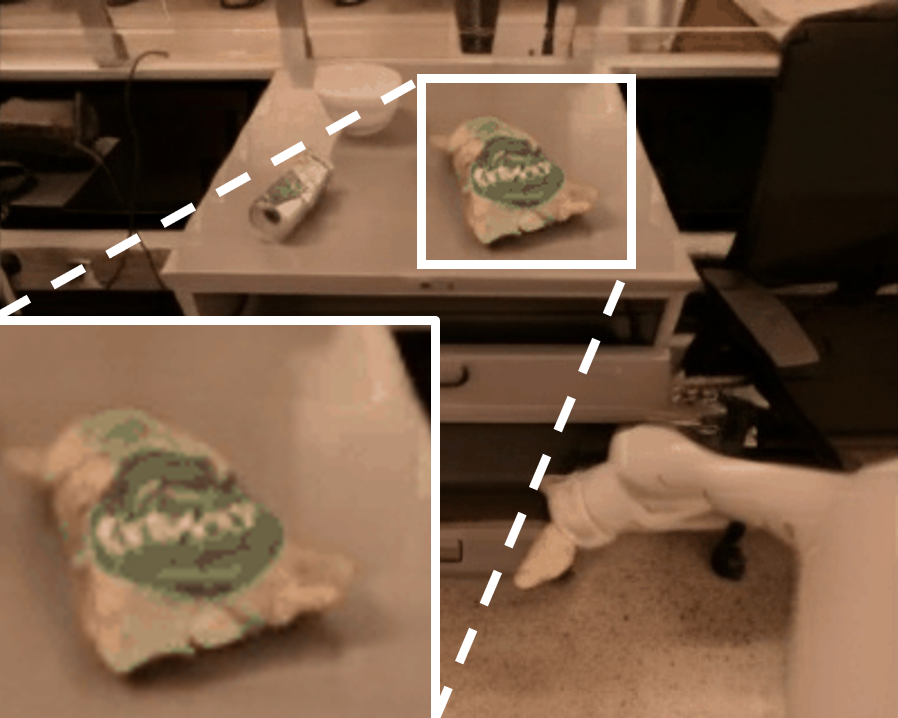
\includegraphics[width=\textwidth]{images/rt1/edited_frames/3-28_avid_final_frame.png}
    \end{minipage}%
    \vspace{0.03cm} % Space between rows
    \begin{minipage}{0.04\textwidth} % Column for rotated method name
        \centering
        \raisebox{0.1\textwidth}{\rotatebox{90}{\textbf{\tiny \shortstack{Action Cond.\\Diffusion 145M }}}}
    \end{minipage}%
    \hfill
    \begin{minipage}{0.155\textwidth}
        \centering
        
\includegraphics[width=\textwidth]{images/rt1/act_cond_diffusion_145M/3-28-samples_frames/frame_0.png}
    \end{minipage}%
    \hfill
    \begin{minipage}{0.155\textwidth}
        \centering
        
\includegraphics[width=\textwidth]{images/rt1/act_cond_diffusion_145M/3-28-samples_frames/frame_3.png}
    \end{minipage}%
    \hfill
    \begin{minipage}{0.155\textwidth}
        \centering
        
\includegraphics[width=\textwidth]{images/rt1/act_cond_diffusion_145M/3-28-samples_frames/frame_6.png}
    \end{minipage}%
    \hfill
    \begin{minipage}{0.155\textwidth}
        \centering
        
\includegraphics[width=\textwidth]{images/rt1/act_cond_diffusion_145M/3-28-samples_frames/frame_9.png}
    \end{minipage}%
    \hfill
    \begin{minipage}{0.155\textwidth}
        \centering
        
\includegraphics[width=\textwidth]{images/rt1/act_cond_diffusion_145M/3-28-samples_frames/frame_12.png}
    \end{minipage}%
    \hfill
    \begin{minipage}{0.155\textwidth}
        \centering
        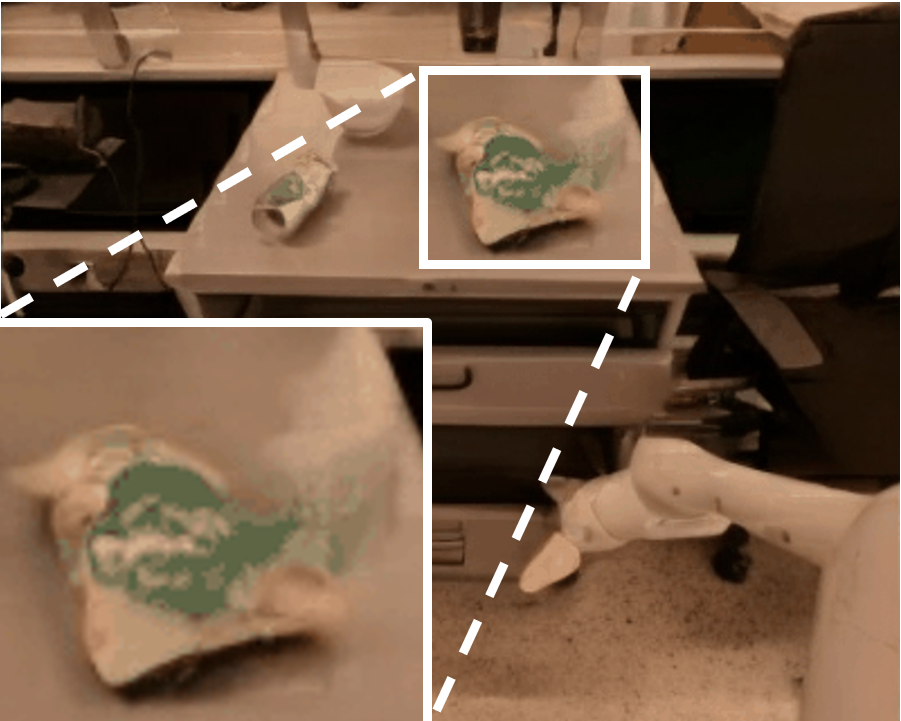
\includegraphics[width=\textwidth]{images/rt1/edited_frames/3028_act_cond_145M_final_frame.png}
    \end{minipage}%
    \vspace{0.03cm} % Space between rows
    \begin{minipage}{0.04\textwidth} % Column for rotated method name
        \centering
        \raisebox{0.1\textwidth}{\rotatebox{90}{\textbf{\tiny \shortstack{DynamiCrafter }}}}
    \end{minipage}%
    \hfill
    \begin{minipage}{0.155\textwidth}
        \centering
        
\includegraphics[width=\textwidth]{images/rt1/dynamicrafter/3-28-samples_frames/frame_0.png}
    \end{minipage}%
    \hfill
    \begin{minipage}{0.155\textwidth}
        \centering
        
\includegraphics[width=\textwidth]{images/rt1/dynamicrafter/3-28-samples_frames/frame_3.png}
    \end{minipage}%
    \hfill
    \begin{minipage}{0.155\textwidth}
        \centering
        
\includegraphics[width=\textwidth]{images/rt1/dynamicrafter/3-28-samples_frames/frame_6.png}
    \end{minipage}%
    \hfill
    \begin{minipage}{0.155\textwidth}
        \centering
        
\includegraphics[width=\textwidth]{images/rt1/dynamicrafter/3-28-samples_frames/frame_9.png}
    \end{minipage}%
    \hfill
    \begin{minipage}{0.155\textwidth}
        \centering
        
\includegraphics[width=\textwidth]{images/rt1/dynamicrafter/3-28-samples_frames/frame_12.png}
    \end{minipage}%
    \hfill
    \begin{minipage}{0.155\textwidth}
        \centering
        
\includegraphics[width=\textwidth]{images/rt1/dynamicrafter/3-28-samples_frames/frame_15.png}
    \end{minipage}%
    \vspace{0.4cm} % Space between rows
    \begin{minipage}{0.04\textwidth} % Column for rotated method name
        \centering
        \raisebox{0.1\textwidth}{\rotatebox{90}{\textbf{\tiny \shortstack{Ground Truth }}}}
    \end{minipage}%
    \hfill
    \begin{minipage}{0.155\textwidth}
        \centering
        
\includegraphics[width=\textwidth]{images/rt1/real_videos/3-329-real_frames/frame_0.png}
    \end{minipage}%
    \hfill
    \begin{minipage}{0.155\textwidth}
        \centering
        
\includegraphics[width=\textwidth]{images/rt1/real_videos/3-329-real_frames/frame_3.png}
    \end{minipage}%
    \hfill
    \begin{minipage}{0.155\textwidth}
        \centering
        
\includegraphics[width=\textwidth]{images/rt1/real_videos/3-329-real_frames/frame_6.png}
    \end{minipage}%
    \hfill
    \begin{minipage}{0.155\textwidth}
        \centering
        
\includegraphics[width=\textwidth]{images/rt1/real_videos/3-329-real_frames/frame_9.png}
    \end{minipage}%
    \hfill
    \begin{minipage}{0.155\textwidth}
        \centering
        
\includegraphics[width=\textwidth]{images/rt1/real_videos/3-329-real_frames/frame_12.png}
    \end{minipage}%
    \hfill
    \begin{minipage}{0.155\textwidth}
        \centering
        
\includegraphics[width=\textwidth]{images/rt1/real_videos/3-329-real_frames/frame_15.png}
    \end{minipage}%
    \vspace{0.03cm} % Space between rows
    \begin{minipage}{0.04\textwidth} % Column for rotated method name
        \centering
        \raisebox{0.1\textwidth}{\rotatebox{90}{\textbf{\tiny \shortstack{AVID 145M}}}}
    \end{minipage}%
    \hfill
    \begin{minipage}{0.155\textwidth}
        \centering
        
\includegraphics[width=\textwidth]{images/rt1/avid_145M/3-329-samples_frames/frame_0.png}
    \end{minipage}%
    \hfill
    \begin{minipage}{0.155\textwidth}
        \centering
        
\includegraphics[width=\textwidth]{images/rt1/avid_145M/3-329-samples_frames/frame_3.png}
    \end{minipage}%
    \hfill
    \begin{minipage}{0.155\textwidth}
        \centering
        
\includegraphics[width=\textwidth]{images/rt1/avid_145M/3-329-samples_frames/frame_6.png}
    \end{minipage}%
    \hfill
    \begin{minipage}{0.155\textwidth}
        \centering
        
\includegraphics[width=\textwidth]{images/rt1/avid_145M/3-329-samples_frames/frame_9.png}
    \end{minipage}%
    \hfill
    \begin{minipage}{0.155\textwidth}
        \centering
        
\includegraphics[width=\textwidth]{images/rt1/avid_145M/3-329-samples_frames/frame_12.png}
    \end{minipage}%
    \hfill
    \begin{minipage}{0.155\textwidth}
        \centering
        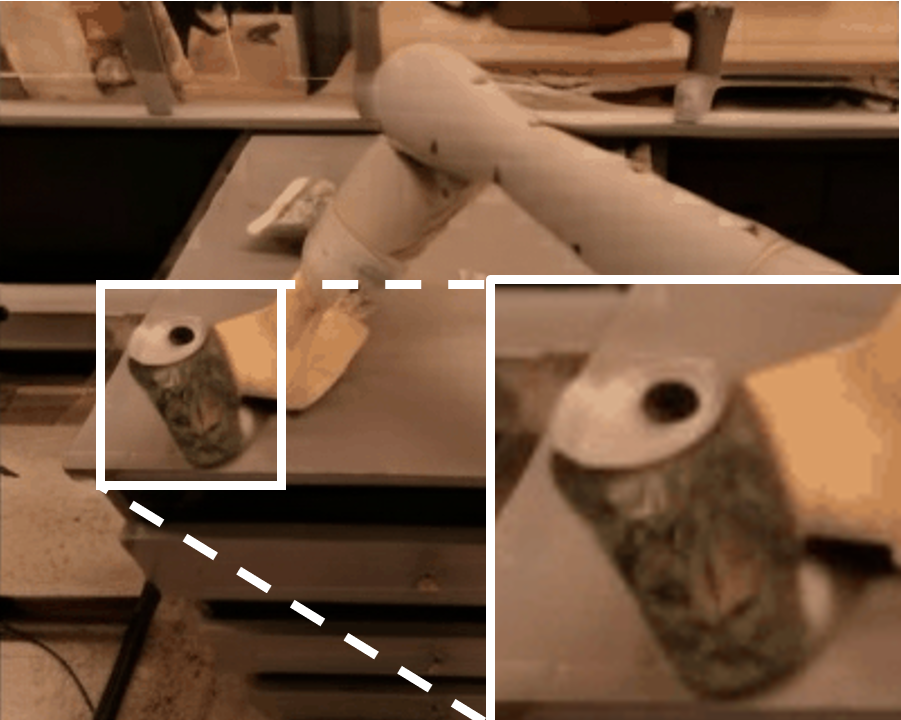
\includegraphics[width=\textwidth]{images/rt1/edited_frames/3-329_avid_final_frame.png}
    \end{minipage}%
    \vspace{0.03cm} % Space between rows
    \begin{minipage}{0.04\textwidth} % Column for rotated method name
        \centering
        \raisebox{0.1\textwidth}{\rotatebox{90}{\textbf{\tiny \shortstack{Action Cond.\\Diffusion 145M }}}}
    \end{minipage}%
    \hfill
    \begin{minipage}{0.155\textwidth}
        \centering
        
\includegraphics[width=\textwidth]{images/rt1/act_cond_diffusion_145M/3-329-samples_frames/frame_0.png}
    \end{minipage}%
    \hfill
    \begin{minipage}{0.155\textwidth}
        \centering
        
\includegraphics[width=\textwidth]{images/rt1/act_cond_diffusion_145M/3-329-samples_frames/frame_3.png}
    \end{minipage}%
    \hfill
    \begin{minipage}{0.155\textwidth}
        \centering
        
\includegraphics[width=\textwidth]{images/rt1/act_cond_diffusion_145M/3-329-samples_frames/frame_6.png}
    \end{minipage}%
    \hfill
    \begin{minipage}{0.155\textwidth}
        \centering
        
\includegraphics[width=\textwidth]{images/rt1/act_cond_diffusion_145M/3-329-samples_frames/frame_9.png}
    \end{minipage}%
    \hfill
    \begin{minipage}{0.155\textwidth}
        \centering
        
\includegraphics[width=\textwidth]{images/rt1/act_cond_diffusion_145M/3-329-samples_frames/frame_12.png}
    \end{minipage}%
    \hfill
    \begin{minipage}{0.155\textwidth}
        \centering
        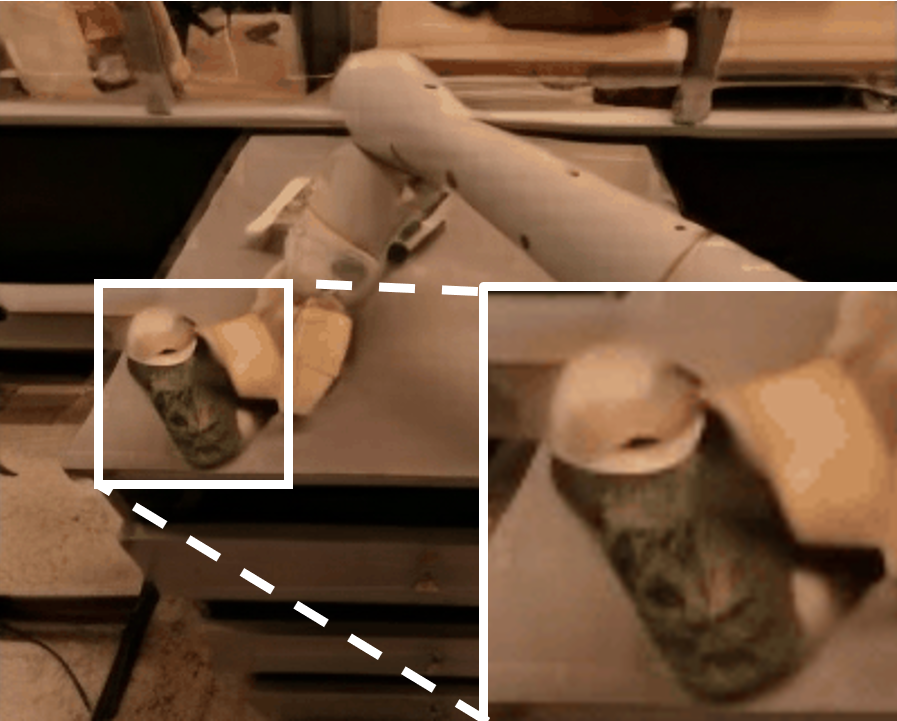
\includegraphics[width=\textwidth]{images/rt1/edited_frames/3-329_act_cond_145M_final_frame.png}
    \end{minipage}%
    \caption{Extended qualitative comparison of videos generated for RT1. \label{fig:qual_extended}}
\end{figure}




\begin{figure}[htbp]
    \begin{minipage}{0.05\textwidth} % Column for rotated method name
        \centering
        \raisebox{0.3\textwidth}{\rotatebox{90}{\textbf{\tiny Ground Truth}}} % Rotating and vertically centering method name
    \end{minipage}%
    \hfill
    \begin{minipage}{0.13\textwidth}
        \centering
        
\includegraphics[width=\textwidth]{images/coinrun/real_videos/3-424_frames/frame_0.png}
    \end{minipage}%
    \hfill
    \begin{minipage}{0.13\textwidth}
        \centering
        
\includegraphics[width=\textwidth]{images/coinrun/real_videos/3-424_frames/frame_2.png}
    \end{minipage}%
    \hfill
    \begin{minipage}{0.13\textwidth}
        \centering
        
\includegraphics[width=\textwidth]{images/coinrun/real_videos/3-424_frames/frame_3.png}
    \end{minipage}%
    \hfill
    \begin{minipage}{0.13\textwidth}
        \centering
        
\includegraphics[width=\textwidth]{images/coinrun/real_videos/3-424_frames/frame_5.png}
    \end{minipage}%
    \hfill
    \begin{minipage}{0.13\textwidth}
        \centering
        
\includegraphics[width=\textwidth]{images/coinrun/real_videos/3-424_frames/frame_6.png}
    \end{minipage}%
    \hfill
    \begin{minipage}{0.13\textwidth}
        \centering
        
\includegraphics[width=\textwidth]{images/coinrun/real_videos/3-424_frames/frame_8.png}
    \end{minipage}%
    \hfill
    \begin{minipage}{0.13\textwidth}
        \centering
        
\includegraphics[width=\textwidth]{images/coinrun/real_videos/3-424_frames/frame_9.png}
    \end{minipage}%
    \vspace{0.01cm}
    %
    \begin{minipage}{0.05\textwidth} % Column for rotated method name
        \centering
        \raisebox{0.3\textwidth}{\rotatebox{90}{\textbf{\tiny AVID 71M}}} % Rotating and vertically centering method name
    \end{minipage}%
    \hfill
    \begin{minipage}{0.13\textwidth}
        \centering
        
\includegraphics[width=\textwidth]{images/coinrun/avid_71M/3-424_frames/frame_0.png}
    \end{minipage}%
    \hfill
    \begin{minipage}{0.13\textwidth}
        \centering
        
\includegraphics[width=\textwidth]{images/coinrun/avid_71M/3-424_frames/frame_2.png}
    \end{minipage}%
    \hfill
    \begin{minipage}{0.13\textwidth}
        \centering
        
\includegraphics[width=\textwidth]{images/coinrun/avid_71M/3-424_frames/frame_3.png}
    \end{minipage}%
    \hfill
    \begin{minipage}{0.13\textwidth}
        \centering
        
\includegraphics[width=\textwidth]{images/coinrun/avid_71M/3-424_frames/frame_5.png}
    \end{minipage}%
    \hfill
    \begin{minipage}{0.13\textwidth}
        \centering
        
\includegraphics[width=\textwidth]{images/coinrun/avid_71M/3-424_frames/frame_6.png}
    \end{minipage}%
    \hfill
    \begin{minipage}{0.13\textwidth}
        \centering
        
\includegraphics[width=\textwidth]{images/coinrun/avid_71M/3-424_frames/frame_8.png}
    \end{minipage}%
    \hfill
    \begin{minipage}{0.13\textwidth}
        \centering
        
\includegraphics[width=\textwidth]{images/coinrun/avid_71M/3-424_frames/frame_9.png}
    \end{minipage}%
    \vspace{0.01cm}
    %
    \begin{minipage}{0.05\textwidth} % Column for rotated method name
        \centering
        \raisebox{0.1\textwidth}{\rotatebox{90}{\textbf{\tiny \shortstack{Action Cond.\\Diffusion 71M }}}}
    \end{minipage}%
    \hfill
    \begin{minipage}{0.13\textwidth}
        \centering
        
\includegraphics[width=\textwidth]{images/coinrun/act_cond_diffusion_71M/3-424_frames/frame_0.png}
    \end{minipage}%
    \hfill
    \begin{minipage}{0.13\textwidth}
        \centering
        
\includegraphics[width=\textwidth]{images/coinrun/act_cond_diffusion_71M/3-424_frames/frame_2.png}
    \end{minipage}%
    \hfill
    \begin{minipage}{0.13\textwidth}
        \centering
        
\includegraphics[width=\textwidth]{images/coinrun/act_cond_diffusion_71M/3-424_frames/frame_3.png}
    \end{minipage}%
    \hfill
    \begin{minipage}{0.13\textwidth}
        \centering
        
\includegraphics[width=\textwidth]{images/coinrun/act_cond_diffusion_71M/3-424_frames/frame_5.png}
    \end{minipage}%
    \hfill
    \begin{minipage}{0.13\textwidth}
        \centering
        
\includegraphics[width=\textwidth]{images/coinrun/act_cond_diffusion_71M/3-424_frames/frame_6.png}
    \end{minipage}%
    \hfill
    \begin{minipage}{0.13\textwidth}
        \centering
        
\includegraphics[width=\textwidth]{images/coinrun/act_cond_diffusion_71M/3-424_frames/frame_8.png}
    \end{minipage}%
    \hfill
    \begin{minipage}{0.13\textwidth}
        \centering
        
\includegraphics[width=\textwidth]{images/coinrun/act_cond_diffusion_71M/3-424_frames/frame_9.png}
    \end{minipage}%
    \vspace{0.01cm}
    %
    \begin{minipage}{0.05\textwidth} % Column for rotated method name
        \centering
        \raisebox{0.1\textwidth}{\rotatebox{90}{\tiny \textbf{Pretrained Model }}}
    \end{minipage}%
    \hfill
    \begin{minipage}{0.13\textwidth}
        \centering
        
\includegraphics[width=\textwidth]{images/coinrun/base_model/3-424_frames/frame_0.png}
    \end{minipage}%
    \hfill
    \begin{minipage}{0.13\textwidth}
        \centering
        
\includegraphics[width=\textwidth]{images/coinrun/base_model/3-424_frames/frame_2.png}
    \end{minipage}%
    \hfill
    \begin{minipage}{0.13\textwidth}
        \centering
        
\includegraphics[width=\textwidth]{images/coinrun/base_model/3-424_frames/frame_3.png}
    \end{minipage}%
    \hfill
    \begin{minipage}{0.13\textwidth}
        \centering
        
\includegraphics[width=\textwidth]{images/coinrun/base_model/3-424_frames/frame_5.png}
    \end{minipage}%
    \hfill
    \begin{minipage}{0.13\textwidth}
        \centering
        
\includegraphics[width=\textwidth]{images/coinrun/base_model/3-424_frames/frame_6.png}
    \end{minipage}%
    \hfill
    \begin{minipage}{0.13\textwidth}
        \centering
        
\includegraphics[width=\textwidth]{images/coinrun/base_model/3-424_frames/frame_8.png}
    \end{minipage}%
    \hfill
    \begin{minipage}{0.13\textwidth}
        \centering
        
\includegraphics[width=\textwidth]{images/coinrun/base_model/3-424_frames/frame_9.png}
    \end{minipage}%
    %
    %
    %
    \vspace{0.3cm}
    %
    %
     \begin{minipage}{0.05\textwidth} % Column for rotated method name
        \centering
        \raisebox{0.3\textwidth}{\rotatebox{90}{\textbf{\tiny Ground Truth}}} % Rotating and vertically centering method name
    \end{minipage}%
    \hfill
    \begin{minipage}{0.13\textwidth}
        \centering
        
\includegraphics[width=\textwidth]{images/coinrun/real_videos/5-1369_frames/frame_0.png}
    \end{minipage}%
    \hfill
    \begin{minipage}{0.13\textwidth}
        \centering
        
\includegraphics[width=\textwidth]{images/coinrun/real_videos/5-1369_frames/frame_2.png}
    \end{minipage}%
    \hfill
    \begin{minipage}{0.13\textwidth}
        \centering
        
\includegraphics[width=\textwidth]{images/coinrun/real_videos/5-1369_frames/frame_3.png}
    \end{minipage}%
    \hfill
    \begin{minipage}{0.13\textwidth}
        \centering
        
\includegraphics[width=\textwidth]{images/coinrun/real_videos/5-1369_frames/frame_5.png}
    \end{minipage}%
    \hfill
    \begin{minipage}{0.13\textwidth}
        \centering
        
\includegraphics[width=\textwidth]{images/coinrun/real_videos/5-1369_frames/frame_6.png}
    \end{minipage}%
    \hfill
    \begin{minipage}{0.13\textwidth}
        \centering
        
\includegraphics[width=\textwidth]{images/coinrun/real_videos/5-1369_frames/frame_8.png}
    \end{minipage}%
    \hfill
    \begin{minipage}{0.13\textwidth}
        \centering
        
\includegraphics[width=\textwidth]{images/coinrun/real_videos/5-1369_frames/frame_9.png}
    \end{minipage}%
    \vspace{0.01cm}
    %
    \begin{minipage}{0.05\textwidth} % Column for rotated method name
        \centering
        \raisebox{0.3\textwidth}{\rotatebox{90}{\textbf{\tiny AVID 71M}}} % Rotating and vertically centering method name
    \end{minipage}%
    \hfill
    \begin{minipage}{0.13\textwidth}
        \centering
        
\includegraphics[width=\textwidth]{images/coinrun/avid_71M/5-1369_frames/frame_0.png}
    \end{minipage}%
    \hfill
    \begin{minipage}{0.13\textwidth}
        \centering
        
\includegraphics[width=\textwidth]{images/coinrun/avid_71M/5-1369_frames/frame_2.png}
    \end{minipage}%
    \hfill
    \begin{minipage}{0.13\textwidth}
        \centering
        
\includegraphics[width=\textwidth]{images/coinrun/avid_71M/5-1369_frames/frame_3.png}
    \end{minipage}%
    \hfill
    \begin{minipage}{0.13\textwidth}
        \centering
        
\includegraphics[width=\textwidth]{images/coinrun/avid_71M/5-1369_frames/frame_5.png}
    \end{minipage}%
    \hfill
    \begin{minipage}{0.13\textwidth}
        \centering
        
\includegraphics[width=\textwidth]{images/coinrun/avid_71M/5-1369_frames/frame_6.png}
    \end{minipage}%
    \hfill
    \begin{minipage}{0.13\textwidth}
        \centering
        
\includegraphics[width=\textwidth]{images/coinrun/avid_71M/5-1369_frames/frame_8.png}
    \end{minipage}%
    \hfill
    \begin{minipage}{0.13\textwidth}
        \centering
        
\includegraphics[width=\textwidth]{images/coinrun/avid_71M/5-1369_frames/frame_9.png}
    \end{minipage}%
    \vspace{0.01cm}
    %
    \begin{minipage}{0.05\textwidth} % Column for rotated method name
        \centering
        \raisebox{0.1\textwidth}{\rotatebox{90}{\textbf{\tiny \shortstack{Action Cond.\\Diffusion 71M }}}}
    \end{minipage}%
    \hfill
    \begin{minipage}{0.13\textwidth}
        \centering
        
\includegraphics[width=\textwidth]{images/coinrun/act_cond_diffusion_71M/5-1369_frames/frame_0.png}
    \end{minipage}%
    \hfill
    \begin{minipage}{0.13\textwidth}
        \centering
        
\includegraphics[width=\textwidth]{images/coinrun/act_cond_diffusion_71M/5-1369_frames/frame_2.png}
    \end{minipage}%
    \hfill
    \begin{minipage}{0.13\textwidth}
        \centering
        
\includegraphics[width=\textwidth]{images/coinrun/act_cond_diffusion_71M/5-1369_frames/frame_3.png}
    \end{minipage}%
    \hfill
    \begin{minipage}{0.13\textwidth}
        \centering
        
\includegraphics[width=\textwidth]{images/coinrun/act_cond_diffusion_71M/5-1369_frames/frame_5.png}
    \end{minipage}%
    \hfill
    \begin{minipage}{0.13\textwidth}
        \centering
        
\includegraphics[width=\textwidth]{images/coinrun/act_cond_diffusion_71M/5-1369_frames/frame_6.png}
    \end{minipage}%
    \hfill
    \begin{minipage}{0.13\textwidth}
        \centering
        
\includegraphics[width=\textwidth]{images/coinrun/act_cond_diffusion_71M/5-1369_frames/frame_8.png}
    \end{minipage}%
    \hfill
    \begin{minipage}{0.13\textwidth}
        \centering
        
\includegraphics[width=\textwidth]{images/coinrun/act_cond_diffusion_71M/5-1369_frames/frame_9.png}
    \end{minipage}%
    \vspace{0.01cm}
    %
    \begin{minipage}{0.05\textwidth} % Column for rotated method name
        \centering
        \raisebox{0.1\textwidth}{\rotatebox{90}{\tiny \textbf{Pretrained Model }}}
    \end{minipage}%
    \hfill
    \begin{minipage}{0.13\textwidth}
        \centering
        
\includegraphics[width=\textwidth]{images/coinrun/base_model/5-1369_frames/frame_0.png}
    \end{minipage}%
    \hfill
    \begin{minipage}{0.13\textwidth}
        \centering
        
\includegraphics[width=\textwidth]{images/coinrun/base_model/5-1369_frames/frame_2.png}
    \end{minipage}%
    \hfill
    \begin{minipage}{0.13\textwidth}
        \centering
        
\includegraphics[width=\textwidth]{images/coinrun/base_model/5-1369_frames/frame_3.png}
    \end{minipage}%
    \hfill
    \begin{minipage}{0.13\textwidth}
        \centering
        
\includegraphics[width=\textwidth]{images/coinrun/base_model/5-1369_frames/frame_5.png}
    \end{minipage}%
    \hfill
    \begin{minipage}{0.13\textwidth}
        \centering
        
\includegraphics[width=\textwidth]{images/coinrun/base_model/5-1369_frames/frame_6.png}
    \end{minipage}%
    \hfill
    \begin{minipage}{0.13\textwidth}
        \centering
        
\includegraphics[width=\textwidth]{images/coinrun/base_model/5-1369_frames/frame_8.png}
    \end{minipage}%
    \hfill
    \begin{minipage}{0.13\textwidth}
        \centering
        
\includegraphics[width=\textwidth]{images/coinrun/base_model/5-1369_frames/frame_9.png}
    \end{minipage}%
    %
    %
    %
    \vspace{0.3cm}
    %
    %
    \begin{minipage}{0.05\textwidth} % Column for rotated method name
        \centering
        \raisebox{0.3\textwidth}{\rotatebox{90}{\textbf{\tiny Ground Truth}}} % Rotating and vertically centering method name
    \end{minipage}%
    \hfill
    \begin{minipage}{0.13\textwidth}
        \centering
        \includegraphics[width=\textwidth]{images/coinrun/real_videos/2-837_frames/frame_0.png}
    \end{minipage}%
    \hfill
    \begin{minipage}{0.13\textwidth}
        \centering
        
\includegraphics[width=\textwidth]{images/coinrun/real_videos/2-837_frames/frame_2.png}
    \end{minipage}%
    \hfill
    \begin{minipage}{0.13\textwidth}
        \centering
        
\includegraphics[width=\textwidth]{images/coinrun/real_videos/2-837_frames/frame_3.png}
    \end{minipage}%
    \hfill
    \begin{minipage}{0.13\textwidth}
        \centering
        
\includegraphics[width=\textwidth]{images/coinrun/real_videos/2-837_frames/frame_5.png}
    \end{minipage}%
    \hfill
    \begin{minipage}{0.13\textwidth}
        \centering
        
\includegraphics[width=\textwidth]{images/coinrun/real_videos/2-837_frames/frame_6.png}
    \end{minipage}%
    \hfill
    \begin{minipage}{0.13\textwidth}
        \centering
        
\includegraphics[width=\textwidth]{images/coinrun/real_videos/2-837_frames/frame_8.png}
    \end{minipage}%
    \hfill
    \begin{minipage}{0.13\textwidth}
        \centering
        
\includegraphics[width=\textwidth]{images/coinrun/real_videos/2-837_frames/frame_9.png}
    \end{minipage}%
     %
    \vspace{0.01cm}
    %
    \begin{minipage}{0.05\textwidth} % Column for rotated method name
        \centering
        \raisebox{0.3\textwidth}{\rotatebox{90}{\textbf{\tiny AVID 71M}}} % Rotating and vertically centering method name
    \end{minipage}%
    \hfill
    \begin{minipage}{0.13\textwidth}
        \centering
        
\includegraphics[width=\textwidth]{images/coinrun/avid_71M/2-837_frames/frame_0.png}
    \end{minipage}%
    \hfill
    \begin{minipage}{0.13\textwidth}
        \centering
        
\includegraphics[width=\textwidth]{images/coinrun/avid_71M/2-837_frames/frame_2.png}
    \end{minipage}%
    \hfill
    \begin{minipage}{0.13\textwidth}
        \centering
        
\includegraphics[width=\textwidth]{images/coinrun/avid_71M/2-837_frames/frame_3.png}
    \end{minipage}%
    \hfill
    \begin{minipage}{0.13\textwidth}
        \centering
        
\includegraphics[width=\textwidth]{images/coinrun/avid_71M/2-837_frames/frame_5.png}
    \end{minipage}%
    \hfill
    \begin{minipage}{0.13\textwidth}
        \centering
        
\includegraphics[width=\textwidth]{images/coinrun/avid_71M/2-837_frames/frame_6.png}
    \end{minipage}%
    \hfill
    \begin{minipage}{0.13\textwidth}
        \centering
        
\includegraphics[width=\textwidth]{images/coinrun/avid_71M/2-837_frames/frame_8.png}
    \end{minipage}%
    \hfill
    \begin{minipage}{0.13\textwidth}
        \centering
        
\includegraphics[width=\textwidth]{images/coinrun/avid_71M/2-837_frames/frame_9.png}
    \end{minipage}%
     %
    \vspace{0.01cm}
    %
    \begin{minipage}{0.05\textwidth} % Column for rotated method name
        \centering
         \raisebox{0.1\textwidth}{\rotatebox{90}{\textbf{\tiny \shortstack{Action Cond.\\Diffusion 71M }}}}
    \end{minipage}%
    \hfill
    \begin{minipage}{0.13\textwidth}
        \centering
        \includegraphics[width=\textwidth]{images/coinrun/act_cond_diffusion_71M/2-837_frames/frame_0.png}
    \end{minipage}%
    \hfill
    \begin{minipage}{0.13\textwidth}
        \centering
        
\includegraphics[width=\textwidth]{images/coinrun/act_cond_diffusion_71M/2-837_frames/frame_2.png}
    \end{minipage}%
    \hfill
    \begin{minipage}{0.13\textwidth}
        \centering
        
\includegraphics[width=\textwidth]{images/coinrun/act_cond_diffusion_71M/2-837_frames/frame_3.png}
    \end{minipage}%
    \hfill
    \begin{minipage}{0.13\textwidth}
        \centering
        
\includegraphics[width=\textwidth]{images/coinrun/act_cond_diffusion_71M/2-837_frames/frame_5.png}
    \end{minipage}%
    \hfill
    \begin{minipage}{0.13\textwidth}
        \centering
        
\includegraphics[width=\textwidth]{images/coinrun/act_cond_diffusion_71M/2-837_frames/frame_6.png}
    \end{minipage}%
    \hfill
    \begin{minipage}{0.13\textwidth}
        \centering
        
\includegraphics[width=\textwidth]{images/coinrun/act_cond_diffusion_71M/2-837_frames/frame_8.png}
    \end{minipage}%
    \hfill
    \begin{minipage}{0.13\textwidth}
        \centering
        
\includegraphics[width=\textwidth]{images/coinrun/act_cond_diffusion_71M/2-837_frames/frame_9.png}
    \end{minipage}%
     %
    \vspace{0.01cm}
    %
    \begin{minipage}{0.05\textwidth} % Column for rotated method name
        \centering
        \raisebox{0.3\textwidth}{\rotatebox{90}{\textbf{\tiny Pretrained Model}}} % Rotating and vertically centering method name
    \end{minipage}%
    \hfill
    \begin{minipage}{0.13\textwidth}
        \centering
        \includegraphics[width=\textwidth]{images/coinrun/base_model/2-837_frames/frame_0.png}
    \end{minipage}%
    \hfill
    \begin{minipage}{0.13\textwidth}
        \centering
        
\includegraphics[width=\textwidth]{images/coinrun/base_model/2-837_frames/frame_2.png}
    \end{minipage}%
    \hfill
    \begin{minipage}{0.13\textwidth}
        \centering
        
\includegraphics[width=\textwidth]{images/coinrun/base_model/2-837_frames/frame_3.png}
    \end{minipage}%
    \hfill
    \begin{minipage}{0.13\textwidth}
        \centering
        
\includegraphics[width=\textwidth]{images/coinrun/base_model/2-837_frames/frame_5.png}
    \end{minipage}%
    \hfill
    \begin{minipage}{0.13\textwidth}
        \centering
        
\includegraphics[width=\textwidth]{images/coinrun/base_model/2-837_frames/frame_6.png}
    \end{minipage}%
    \hfill
    \begin{minipage}{0.13\textwidth}
        \centering
        \includegraphics[width=\textwidth]{images/coinrun/base_model/2-837_frames/frame_8.png}
    \end{minipage}%
    \hfill
    \begin{minipage}{0.13\textwidth}
        \centering
        \includegraphics[width=\textwidth]{images/coinrun/base_model/2-837_frames/frame_9.png}
    \end{minipage}%
    \caption{Extended qualitative comparison of videos generated for Coinrun 500k. \label{fig:procgen_qualitative_extended}}
\end{figure}

\FloatBarrier


\subsection{Example Videos with Same Initial Frame}
\label{app:different_actions}
In Figure~\ref{fig:fixed_actions} we generate videos by providing the same initial conditioning frame but different actions. The provided action is fixed for all 16 steps of the video.
\begin{figure}[htbp]
    \centering
    % Row 1
    \begin{minipage}{0.04\textwidth} % Column for rotated method name
        \centering
        \raisebox{0.3\textwidth}{\rotatebox{90}{\textbf{\tiny Forward}}} % Rotating and vertically centering method name
    \end{minipage}%
    \hfill
    \begin{minipage}{0.155\textwidth}
        \centering
        \includegraphics[width=\textwidth]{images/rt1_fixed_action/forward/1-14-samples_frames/frame_0.png}
    \end{minipage}%
    \hfill
    \begin{minipage}{0.155\textwidth}
        \centering
        \includegraphics[width=\textwidth]{images/rt1_fixed_action/forward/1-14-samples_frames/frame_3.png}
    \end{minipage}%
    \hfill
    \begin{minipage}{0.155\textwidth}
        \centering
        \includegraphics[width=\textwidth]{images/rt1_fixed_action/forward/1-14-samples_frames/frame_6.png}
    \end{minipage}%
    \hfill
    \begin{minipage}{0.155\textwidth}
        \centering
        \includegraphics[width=\textwidth]{images/rt1_fixed_action/forward/1-14-samples_frames/frame_9.png}
    \end{minipage}%
    \hfill
    \begin{minipage}{0.155\textwidth}
        \centering
        \includegraphics[width=\textwidth]{images/rt1_fixed_action/forward/1-14-samples_frames/frame_12.png}
    \end{minipage}%
    \hfill
    \begin{minipage}{0.155\textwidth}
        \centering
        \includegraphics[width=\textwidth]{images/rt1_fixed_action/forward/1-14-samples_frames/frame_15.png}
    \end{minipage}%
    \vspace{0.03cm} % Space between rows
   \begin{minipage}{0.04\textwidth} % Column for rotated method name
        \centering
        \raisebox{0.3\textwidth}{\rotatebox{90}{\textbf{\tiny Upwards}}} % Rotating and vertically centering method name
    \end{minipage}%
    \hfill
    \begin{minipage}{0.155\textwidth}
        \centering
        \includegraphics[width=\textwidth]{images/rt1_fixed_action/up/1-14-samples_frames/frame_0.png}
    \end{minipage}%
    \hfill
    \begin{minipage}{0.155\textwidth}
        \centering
        \includegraphics[width=\textwidth]{images/rt1_fixed_action/up/1-14-samples_frames/frame_3.png}
    \end{minipage}%
    \hfill
    \begin{minipage}{0.155\textwidth}
        \centering
        \includegraphics[width=\textwidth]{images/rt1_fixed_action/up/1-14-samples_frames/frame_6.png}
    \end{minipage}%
    \hfill
    \begin{minipage}{0.155\textwidth}
        \centering
        \includegraphics[width=\textwidth]{images/rt1_fixed_action/up/1-14-samples_frames/frame_9.png}
    \end{minipage}%
    \hfill
    \begin{minipage}{0.155\textwidth}
        \centering
        \includegraphics[width=\textwidth]{images/rt1_fixed_action/up/1-14-samples_frames/frame_12.png}
    \end{minipage}%
    \hfill
    \begin{minipage}{0.155\textwidth}
        \centering
        \includegraphics[width=\textwidth]{images/rt1_fixed_action/up/1-14-samples_frames/frame_15.png}
    \end{minipage}%
    \vspace{0.2cm} % Space between rows
    \begin{minipage}{0.04\textwidth} % Column for rotated method name
        \centering
        \raisebox{0.3\textwidth}{\rotatebox{90}{\textbf{\tiny Right}}} % Rotating and vertically centering method name
    \end{minipage}%
    \hfill
    \begin{minipage}{0.155\textwidth}
        \centering
        \includegraphics[width=\textwidth]{images/rt1_fixed_action/right/1-21-samples_frames/frame_0.png}
    \end{minipage}%
    \hfill
    \begin{minipage}{0.155\textwidth}
        \centering
        \includegraphics[width=\textwidth]{images/rt1_fixed_action/right/1-21-samples_frames/frame_3.png}
    \end{minipage}%
    \hfill
    \begin{minipage}{0.155\textwidth}
        \centering
        \includegraphics[width=\textwidth]{images/rt1_fixed_action/right/1-21-samples_frames/frame_6.png}
    \end{minipage}%
    \hfill
    \begin{minipage}{0.155\textwidth}
        \centering
        \includegraphics[width=\textwidth]{images/rt1_fixed_action/right/1-21-samples_frames/frame_9.png}
    \end{minipage}%
    \hfill
    \begin{minipage}{0.155\textwidth}
        \centering
        \includegraphics[width=\textwidth]{images/rt1_fixed_action/right/1-21-samples_frames/frame_12.png}
    \end{minipage}%
    \hfill
    \begin{minipage}{0.155\textwidth}
        \centering
        \includegraphics[width=\textwidth]{images/rt1_fixed_action/right/1-21-samples_frames/frame_15.png}
    \end{minipage}%
    \vspace{0.03cm} % Space between rows
   \begin{minipage}{0.04\textwidth} % Column for rotated method name
        \centering
        \raisebox{0.3\textwidth}{\rotatebox{90}{\textbf{\tiny Upwards}}} % Rotating and vertically centering method name
    \end{minipage}%
    \hfill
    \begin{minipage}{0.155\textwidth}
        \centering
        \includegraphics[width=\textwidth]{images/rt1_fixed_action/up/1-21-samples_frames/frame_0.png}
    \end{minipage}%
    \hfill
    \begin{minipage}{0.155\textwidth}
        \centering
        \includegraphics[width=\textwidth]{images/rt1_fixed_action/up/1-21-samples_frames/frame_3.png}
    \end{minipage}%
    \hfill
    \begin{minipage}{0.155\textwidth}
        \centering
        \includegraphics[width=\textwidth]{images/rt1_fixed_action/up/1-21-samples_frames/frame_6.png}
    \end{minipage}%
    \hfill
    \begin{minipage}{0.155\textwidth}
        \centering
        \includegraphics[width=\textwidth]{images/rt1_fixed_action/up/1-21-samples_frames/frame_9.png}
    \end{minipage}%
    \hfill
    \begin{minipage}{0.155\textwidth}
        \centering
        \includegraphics[width=\textwidth]{images/rt1_fixed_action/up/1-21-samples_frames/frame_12.png}
    \end{minipage}%
    \hfill
    \begin{minipage}{0.155\textwidth}
        \centering
        \includegraphics[width=\textwidth]{images/rt1_fixed_action/up/1-21-samples_frames/frame_15.png}
    \end{minipage}%
    \caption{Examples of videos generated for RT1 with same initial frame but different actions.~\label{fig:fixed_actions}}
\end{figure}



\section{Experiment Details}



\subsection{Dataset Details}
\label{sec:dataset_details}

\paragraph{Procgen Pretrained Model Dataset}
The pretrained model is trained on videos sampled from 15 out of the 16 procedurally generated games of Procgen, excluding the 16th game Coinrun. Because the games are procedurally generated, each level in each Procgen game has different visual characteristics. To generate the dataset for the pretrained model, in each of the 15 games we sample an episode of 1000 steps long from each of the first 2000 levels by executing uniformly random actions. This results in 2M frames from each game for a total dataset of 30M steps, each with a resolution of $64 \times 64$. For training, we sample windows of 10 steps from the episodes. The pretrained model is trained on videos from this dataset for 12 days in a single A100.

\begin{figure}[htbp]
    \centering
    \begin{minipage}{0.14\textwidth}
        \centering
        \includegraphics[width=\textwidth]{images/procgen_base/1-12000_frames/frame_0.png}
    \end{minipage}%
    \hfill
    \begin{minipage}{0.14\textwidth}
        \centering
        \includegraphics[width=\textwidth]{images/procgen_base/1-12000_frames/frame_2.png}
    \end{minipage}%
    \hfill
    \begin{minipage}{0.14\textwidth}
        \centering
        \includegraphics[width=\textwidth]{images/procgen_base/1-12000_frames/frame_3.png}
    \end{minipage}%
    \hfill
    \begin{minipage}{0.14\textwidth}
        \centering
        \includegraphics[width=\textwidth]{images/procgen_base/1-12000_frames/frame_5.png}
    \end{minipage}%
    \hfill
    \begin{minipage}{0.14\textwidth}
        \centering
        \includegraphics[width=\textwidth]{images/procgen_base/1-12000_frames/frame_6.png}
    \end{minipage}%
    \hfill
    \begin{minipage}{0.14\textwidth}
        \centering
        \includegraphics[width=\textwidth]{images/procgen_base/1-12000_frames/frame_8.png}
    \end{minipage}%
    \hfill
    \begin{minipage}{0.14\textwidth}
        \centering
        \includegraphics[width=\textwidth]{images/procgen_base/1-12000_frames/frame_9.png}
    \end{minipage}%
     \vspace{0.4mm}
    \begin{minipage}{0.14\textwidth}
        \centering
        \includegraphics[width=\textwidth]{images/procgen_base/1-9494_frames/frame_0.png}
    \end{minipage}%
    \hfill
    \begin{minipage}{0.14\textwidth}
        \centering
        \includegraphics[width=\textwidth]{images/procgen_base/1-9494_frames/frame_2.png}
    \end{minipage}%
    \hfill
    \begin{minipage}{0.14\textwidth}
        \centering
        \includegraphics[width=\textwidth]{images/procgen_base/1-9494_frames/frame_3.png}
    \end{minipage}%
    \hfill
    \begin{minipage}{0.14\textwidth}
        \centering
        \includegraphics[width=\textwidth]{images/procgen_base/1-9494_frames/frame_5.png}
    \end{minipage}%
    \hfill
    \begin{minipage}{0.14\textwidth}
        \centering
        \includegraphics[width=\textwidth]{images/procgen_base/1-9494_frames/frame_6.png}
    \end{minipage}%
    \hfill
    \begin{minipage}{0.14\textwidth}
        \centering
        \includegraphics[width=\textwidth]{images/procgen_base/1-9494_frames/frame_8.png}
    \end{minipage}%
    \hfill
    \begin{minipage}{0.14\textwidth}
        \centering
        \includegraphics[width=\textwidth]{images/procgen_base/1-9494_frames/frame_9.png}
    \end{minipage}%
     \vspace{0.4mm}
    \begin{minipage}{0.14\textwidth}
        \centering
        \includegraphics[width=\textwidth]{images/procgen_base/1-6272_frames/frame_0.png}
    \end{minipage}%
    \hfill
    \begin{minipage}{0.14\textwidth}
        \centering
        \includegraphics[width=\textwidth]{images/procgen_base/1-6272_frames/frame_2.png}
    \end{minipage}%
    \hfill
    \begin{minipage}{0.14\textwidth}
        \centering
        \includegraphics[width=\textwidth]{images/procgen_base/1-6272_frames/frame_3.png}
    \end{minipage}%
    \hfill
    \begin{minipage}{0.14\textwidth}
        \centering
        \includegraphics[width=\textwidth]{images/procgen_base/1-6272_frames/frame_5.png}
    \end{minipage}%
    \hfill
    \begin{minipage}{0.14\textwidth}
        \centering
        \includegraphics[width=\textwidth]{images/procgen_base/1-6272_frames/frame_6.png}
    \end{minipage}%
    \hfill
    \begin{minipage}{0.14\textwidth}
        \centering
        \includegraphics[width=\textwidth]{images/procgen_base/1-6272_frames/frame_8.png}
    \end{minipage}%
    \hfill
    \begin{minipage}{0.14\textwidth}
        \centering
        \includegraphics[width=\textwidth]{images/procgen_base/1-6272_frames/frame_9.png}
    \end{minipage}%
    \vspace{0.4mm}
    \begin{minipage}{0.14\textwidth}
        \centering
        \includegraphics[width=\textwidth]{images/procgen_base/1-10031_frames/frame_0.png}
    \end{minipage}%
    \hfill
    \begin{minipage}{0.14\textwidth}
        \centering
        \includegraphics[width=\textwidth]{images/procgen_base/1-10031_frames/frame_2.png}
    \end{minipage}%
    \hfill
    \begin{minipage}{0.14\textwidth}
        \centering
        \includegraphics[width=\textwidth]{images/procgen_base/1-10031_frames/frame_3.png}
    \end{minipage}%
    \hfill
    \begin{minipage}{0.14\textwidth}
        \centering
        \includegraphics[width=\textwidth]{images/procgen_base/1-10031_frames/frame_5.png}
    \end{minipage}%
    \hfill
    \begin{minipage}{0.14\textwidth}
        \centering
        \includegraphics[width=\textwidth]{images/procgen_base/1-10031_frames/frame_6.png}
    \end{minipage}%
    \hfill
    \begin{minipage}{0.14\textwidth}
        \centering
        \includegraphics[width=\textwidth]{images/procgen_base/1-10031_frames/frame_8.png}
    \end{minipage}%
    \hfill
    \begin{minipage}{0.14\textwidth}
        \centering
        \includegraphics[width=\textwidth]{images/procgen_base/1-10031_frames/frame_9.png}
    \end{minipage}%
    \vspace{0.4mm}
    \begin{minipage}{0.14\textwidth}
        \centering
        \includegraphics[width=\textwidth]{images/procgen_base/1-18802_frames/frame_0.png}
    \end{minipage}%
    \hfill
    \begin{minipage}{0.14\textwidth}
        \centering
        \includegraphics[width=\textwidth]{images/procgen_base/1-18802_frames/frame_2.png}
    \end{minipage}%
    \hfill
    \begin{minipage}{0.14\textwidth}
        \centering
        \includegraphics[width=\textwidth]{images/procgen_base/1-18802_frames/frame_3.png}
    \end{minipage}%
    \hfill
    \begin{minipage}{0.14\textwidth}
        \centering
        \includegraphics[width=\textwidth]{images/procgen_base/1-18802_frames/frame_5.png}
    \end{minipage}%
    \hfill
    \begin{minipage}{0.14\textwidth}
        \centering
        \includegraphics[width=\textwidth]{images/procgen_base/1-18802_frames/frame_6.png}
    \end{minipage}%
    \hfill
    \begin{minipage}{0.14\textwidth}
        \centering
        \includegraphics[width=\textwidth]{images/procgen_base/1-18802_frames/frame_8.png}
    \end{minipage}%
    \hfill
    \begin{minipage}{0.14\textwidth}
        \centering
        \includegraphics[width=\textwidth]{images/procgen_base/1-18802_frames/frame_9.png}
    \end{minipage}%
    \vspace{0.4mm}
    \begin{minipage}{0.14\textwidth}
        \centering
        \includegraphics[width=\textwidth]{images/procgen_base/1-3408_frames/frame_0.png}
    \end{minipage}%
    \hfill
    \begin{minipage}{0.14\textwidth}
        \centering
        \includegraphics[width=\textwidth]{images/procgen_base/1-3408_frames/frame_2.png}
    \end{minipage}%
    \hfill
    \begin{minipage}{0.14\textwidth}
        \centering
        \includegraphics[width=\textwidth]{images/procgen_base/1-3408_frames/frame_3.png}
    \end{minipage}%
    \hfill
    \begin{minipage}{0.14\textwidth}
        \centering
        \includegraphics[width=\textwidth]{images/procgen_base/1-3408_frames/frame_5.png}
    \end{minipage}%
    \hfill
    \begin{minipage}{0.14\textwidth}
        \centering
        \includegraphics[width=\textwidth]{images/procgen_base/1-3408_frames/frame_6.png}
    \end{minipage}%
    \hfill
    \begin{minipage}{0.14\textwidth}
        \centering
        \includegraphics[width=\textwidth]{images/procgen_base/1-3408_frames/frame_8.png}
    \end{minipage}%
    \hfill
    \begin{minipage}{0.14\textwidth}
        \centering
        \includegraphics[width=\textwidth]{images/procgen_base/1-3408_frames/frame_9.png}
    \end{minipage}%
    \caption{Examples from Procgen pretraining dataset on the 15 out of 16 Procgen games. Note that the pretraining dataset does not include any samples from Coinrun. \label{fig:procgen_dataset}}
\end{figure}

\paragraph{Coinrun Datasets} To train the Coinrun adapters, we generate an action-labelled dataset from the Coinrun game. At each timestep, the action is one of 15 discrete actions corresponding to keypad inputs. We sample episodes of 1000 steps from each of the first 100, 500, or 2500 levels by executing uniform random actions to create the Coinrun100k, Coinrun500k, and Coinrun2.5M datasets. For training, we sample action-labelled trajectories of 10 steps.

For evaluation, we create a held-out evaluation set of ground truth trajectories of videos and actions. We use 1024 ground truth trajectories of 10 steps each, sampled by executing random action sequences in levels sampled uniformly at random between level 10000 and 11000 of Coinrun. We use the same evaluation trajectories for all methods.


\paragraph{RT1 Dataset} The RT1 dataset contains 87212 action-labelled episodes of a robot performing tasks such as picking up and placing objects, with a total of 3.78M steps.
%
The action at each step is a 7 dimensional continuous vector corresponding to the movement and rotation of the end effector and opening or closing of the gripper.
%
The videos have a resolution of $320 \times 512$.
%
For training, we use 95\% of the episodes, equating to 82851 episodes in the training dataset. We sample windows of 16 steps from these episodes for training the models. For evaluation, we use 1024 trajectories of 16 steps each sampled uniformly at random from the held-out test set of 4361 test episodes. We use the same evaluation trajectories for all methods.


\subsection{Model and Training Details}
\label{sec:model_details}

\paragraph{Procgen and Coinrun} For both the pretrained model trained on 15 of the 16 Procgen games, and the adapters trained on the Coinrun datasets, we use the 3D UNet architecture from Video Diffusion Models~\citep{ho2022video} trained on videos of resolution $64 \times 64$. We condition each model on two initial images to allow the initial direction the agent is moving in to be inferred and allow for more accurate video generation. Detailed hyperparameters for each of the models are in Table~\ref{tab:coinrun_hyperparameters}.

\begin{table}[ht]
\small
\centering
\caption{Hyperparameters for models trained on Procgen and Coinrun.}
\vspace{1mm}
\label{tab:coinrun_hyperparameters}
\begin{tabular}{lcc}
\toprule
\textbf{Hyperparameter} & \textbf{Value} & \textbf{Models} \\
\midrule
\multirow{4}{3.5cm}{Base Channels} & 100 & 97M Pretrained Model, ControlNet \\
                        & 90 & 71M \\ 
                        & 50 & 22M, ControlNet-Small 22M \\ \hline
\multirow{3}{3.5cm}{Attention Head Dims} & 64 & 97M Pretrained Model, all ControlNet variants \\ \
                        & 50 & 22M, 71M\\ \hline
\multirow{3}{3.5cm}{Attention Heads} & 8 & 97M Pretrained Model, all ControlNet variants  \\ \
                        & 6 & 71M  \\
                        & 4 & 22M \\ \hline 
\multirow{2}{3.5cm}{Learning Rate}  & 2e-5 & Finetuning  \\
 & 1e-4 & All other models \\ \hline
\multirow{2}{3.5cm}{Training Time} & 12 days & 97M Pretrained Model  \\ 
& 3 days & All other models \\ \hline
Training Hardware & $1\times$ A100 GPU & \multirow{10}{0.1cm}{All} \\
EMA & 0.995 \\
Channel Multipliers & [1, 2, 4, 8] \\
Sequence Length & 10 steps \\
Batch Size & 64 \\
Noise Steps & 200 \\
Inference Steps & 200 \\
Sampling Method & DDPM \\
Prediction Target & $\mathbf{x}_0$ \\
Noise Schedule & Sigmoid \\
\bottomrule
\end{tabular}
\end{table}


\begin{table}[ht]
\small
\centering
\caption{Hyperparameters for models trained on RT1.}
\vspace{1mm}
\label{tab:rt1_hyperparameters}
\begin{tabular}{lcc}
\toprule
\textbf{Hyperparameter} & \textbf{Value} \\
\midrule
\multirow{5}{3cm}{Base Channels} & 320 & 1.4B, ControlNet \\
   & 160 & ControlNet-Small 170M \\ 
   & 96 & 145M \\
   & 64 & 34M, ControlNet-Small 38M \\
   & 32 & 11M, ControlNet-Small 10M \\ \hline
\multirow{2}{3cm}{Attention Head Dims} & 16 & 11M, ControlNet-Small 10M   \\ \
                        & 64 & All other models \\ \hline
\multirow{3}{3cm}{Channel Multipliers} & [1, 2, 4, 4] & 1.4B, 145M, all ControlNet variants\\
 & [1, 1, 2, 3] & 34M \\
 & [1, 2, 3] & 11M \\ \hline
\multirow{2}{3cm}{Learning Rate}  & 2e-5 & Finetuning \\
 & 1e-4 & All other models \\ \hline
 \multirow{1}{3cm}{Attention Heads} & Channels / Attention Head Dims & \multirow{10}{0.1cm}{All} \\ 
Training Time & 7 days \\ 
Training Hardware & $4\times$ A100 GPU \\
EMA & 0.9995 \\
Sequence Length & 16 steps \\
Batch Size & 64 \\
Noise Steps & 1000 \\
Inference Steps & 50 \\
Sampling Method & DDIM \\
Prediction Target & $\mathbf{v}$ \\
Noise Schedule & Linear \\
\bottomrule
\end{tabular}
\end{table}

\paragraph{RT1} The pretrained model is DynamiCrafter~\citep{xing2023dynamicrafter}, a latent video diffusion model.
%
DynamiCrafter is trained to generate videos at a resolution of $320 \times 512$. To accommodate this, we resize and pad the images from the RT1 dataset to this resolution.
%
DynamiCrafter is trained to optionally accept language conditoning. We use an empty language prompt, except in the case where the model is finetuned with language conditioning (see Section~\ref{sec:baselines}).
%
DynamiCrafter uses the 1.4B 3D UNet architecture from~\citep{chen2023videocrafter1} and the autoencoder from Stable Diffusion~\citep{rombach2022high}.

As discussed in Section~\ref{sec:avid}, we
 use the same autoencoder for our AVID adapter, as well as all baselines.
%
For all methods on RT1, we train a 3D UNet with the same architecture as Dynamicrafter from~\citep{chen2023videocrafter1}, but with a reduced number of parameters. 
%
The hyperparameters for each of the models can be found in Table \ref{tab:rt1_hyperparameters}.


\textbf{Parameterisation} We parameterise all models on Procgen and Coinrun to predict the clean video, $\mathbf{x_0}$, meaning that in practice the output of the pretrained model and the adapter output are both predictions of $\mathbf{x_0}$ rather than the noise. DynamiCrafter is trained using the $\mathbf{v}$ prediction target parameterisation~\citep{salimans2022progressive}, so it outputs a prediction of $\mathbf{v}$. We also train all models on the RT1 dataset to predict the $\mathbf{v}$-target. 

\subsection{Action Error Ratio Evaluation Metric Details}
\label{sec:metric_details}

\paragraph{Coinrun} The actions in Coinrun are discrete so to evaluate the Action Error Ratio we first train a classifier to predict the actions. The video is first processed using the encoder part of the 3D Unet architecture that we use for the diffusion model. This encoding is then flattened, and processed by an MLP which outputs a softmax over the 15 possible actions at each step of the video. The classifier is trained using the cross-entropy loss and has 60M total parameters. It is trained on a large dataset of 10M steps: 1000 steps sampled from each of 10,000 levels of Coinrun.

The Action Error Ratio is then computed as the ratio between the accuracy of the action classifier on real videos divided by the accuracy of the classifier on generated videos:

$$
\mathtt{Action Error Ratio (discrete)} = \frac{\mathtt{action\_accuracy(real\_videos)}}{\mathtt{action\_accuracy(generated\_videos)}}
$$

\paragraph{RT1} The actions in RT1 are continuous so we train a regression model to predict the actions. The actions are first normalised to mean zero and unit variance. The video is processed by the encoder part of the 3D UNet architecture and then an MLP which outputs a prediction for the action at each time step. The regression model is trained using the MSE loss on the same 82851 video dataset that we use for training the adapter models, and has 85M parameters.

The Action Error Ratio is then computed as the ratio between the mean absolute error of the action predictions of the regression model on the generated videos compared to the real videos:

$$
\mathtt{Action Error Ratio (continuous)} = \frac{\mathtt{action\_MAE(generated\_videos)}}{\mathtt{action\_MAE(real\_video)}}
$$

\subsection{Normalized Evaluation Metric Details}
\label{app:normalization}
To compute normalized evaluation metrics plotted in Figures~\ref{fig:rt1_perf},~\ref{fig:coinrun500_perf} and~\ref{fig:coinrun_perf}, we first normalize each evaluation metric to between 0 and 1. In RT1, 0 represents the worst performance for each metric across the Small, Medium or Large model sizes for Action-Conditioned Diffusion, 
ControlNet-Small, or AVID. 1 represents the best performance for each metric across these models.
%
In Coinrun, 0 and 1 represent the worst and best performance for each metric across the Medium or Large model sizes for Action-Conditioned Diffusion,  ControlNet/ControlNet-Small, or AVID, across all of the three datasets: Coinrun100k, Coinrun500k, and Coinrun2.5M. 

The minimum and maximum values used for normalization are summarised in Tables~\ref{tab:rt1_norm} and~\ref{tab:coinrun_norm}.


\begin{table}[h]
\small
\centering
\begin{tabular}{lcccccc}
\toprule
\textbf{} &  \textbf{Action Err. Ratio} &
  \textbf{{FVD }} &
  \textbf{{FID}} &
  \textbf{{SSIM}} &
  \textbf{{LPIPS}} &
  \textbf{{PSNR}}  \\
\midrule
\textbf{Minimum} & 1.384 & 24.9 & 3.375 & 0.767 & 0.142 & 22.9 \\
\textbf{Maximum} & 2.640 & 80.4 & 5.329 & 0.842 & 0.226 & 25.3 \\
\bottomrule
\end{tabular}
\caption{Minimum and maximum values for metric normalization in RT1. \label{tab:rt1_norm}}
\end{table}


\begin{table}[h]
\small
\centering
\begin{tabular}{lcccccc}
\toprule
\textbf{} &  \textbf{Action Err. Ratio} &
  \textbf{{FVD }} &
  \textbf{{FID}} &
  \textbf{{SSIM}} &
  \textbf{{LPIPS}} &
  \textbf{{PSNR}}  \\
\midrule
\textbf{Minimum} & 1.154 & 14.5 & 6.44 & 0.487 & 0.120 & 17.2 \\
\textbf{Maximum} & 1.574 & 65.6 & 11.82 & 0.760 & 0.365 & 25.7 \\
\bottomrule
\end{tabular}
\caption{Minimum and maximum values for metric normalization in Coinrun. \label{tab:coinrun_norm}}
\end{table}

If the goal is to maximize the metric, the normalized value of the metric is computed using:
\begin{equation}
    \mathtt{normalized\_value} = \mathtt{(value - min\_value) / (max\_value  - min\_value)}
\end{equation}

If the goal is to minimize the metric, the normalized value of the metric is computed using:
\begin{equation}
    \mathtt{normalized\_value} = 1 - \mathtt{(value - min\_value) / (max\_value  - min\_value)}
\end{equation}

Once the metrics have been normalized, we compute the mean across all 6 normalized metrics. This final value is plotted in Figures~\ref{fig:rt1_perf},~\ref{fig:coinrun500_perf} and~\ref{fig:coinrun_perf}.

\subsection{Baseline Details}
\label{app:baselines}
Here we provide additional details about the baselines that are not included in the main paper.
\begin{itemize}[leftmargin=*, topsep=0pt]
    \item \textit{Language-Conditioned Finetuning} -- the language description that we use is: ``Robot arm performs the task \{$\mathtt{task\_description}$\} " where \{$\mathtt{task\_description}$\} is the description given in the RT1 dataset.
    \item \textit{Classifier Guidance} \citep{dhariwal2021diffusion} -- For the RT1 domain, since the actions are continuous, we discretise each action dimension into 256 bins  uniformly following~\cite{padalkar2023open} to train the classifier. We tune the weight of the guidance within $w \in \{0.003, 0.01, 0.03, 0.1, 0.3 \}$. 
    \item \textit{Product of Experts} -- we tune the weighting of the two models within $\lambda_p \in \{0.2, 0.4, 0.6 \}$. 
    \item \textit{Action Classifier-Free Guidance} -- we tune the weighting within $\lambda_a \in \{0.3, 1.0, 3.0, 10.0 \}$. 
\end{itemize}

For the baselines that require hyperparameter tuning, we sweep over each value of the hyperparameter and choose the value that obtains the best FVD in our evaluation.

